\documentclass[pl,12pt]{aghdpl}
% \documentclass[en,11pt]{aghdpl}  % praca w języku angielskim

% Lista wszystkich języków stanowiących języki pozycji bibliograficznych użytych w pracy.
% (Zgodnie z zasadami tworzenia bibliografii każda pozycja powinna zostać utworzona zgodnie z zasadami języka, w którym dana publikacja została napisana.)
\usepackage[english,polish]{babel}

% Użyj polskiego łamania wyrazów (zamiast domyślnego angielskiego).
\usepackage{polski}

\usepackage[utf8]{inputenc}

% Załączniki

\usepackage[toc, page]{appendix}
\renewcommand\appendixpagename{Załączniki}
\renewcommand\appendixtocname{Załączniki}

% dodatkowe pakiety

\usepackage{mathtools}
\usepackage{amsfonts}
\usepackage{amsmath}
\usepackage{systeme}
\usepackage{amsthm}
\usepackage{graphicx}
\usepackage{float}% do umieszczenia floatów [H]
\usepackage{enumitem}
\setlist{nosep} % or \setlist{noitemsep} to leave space around whole list
\usepackage[bookmarks,hidelinks]{hyperref}

\newcommand{\overbar}[1]{\mkern 1.5mu\overline{\mkern-1.5mu#1\mkern-1.5mu}\mkern 1.5mu}
% Środowisko float do kodu źródłowego \begin{program}

\floatstyle{plaintop}
\ifcsname{chapter}\endcsname%
    \newfloat{program}{!tbh}{lop}[chapter]
\else%
    \newfloat{program}{!tbh}{lop}
\fi
\floatname{program}{Kod źr.}

% Kod poniżej powoduje, że floaty nie wylatują poza granice sekcji

\usepackage{placeins}

\ifcsname{chapter}\endcsname%
    \let\Oldchapter\chapter
    \renewcommand{\chapter}{\FloatBarrier\Oldchapter}
\fi

\let\Oldsection\section
\renewcommand{\section}{\FloatBarrier\Oldsection}

\let\Oldsubsection\subsection
\renewcommand{\subsection}{\FloatBarrier\Oldsubsection}

\let\Oldsubsubsection\subsubsection
\renewcommand{\subsubsection}{\FloatBarrier\Oldsubsubsection}

% --- < bibliografia > ---


\usepackage[
style=numeric,
sorting=none,
%
% Zastosuj styl wpisu bibliograficznego właściwy językowi publikacji.
language=autobib,
autolang=other,
% Zapisuj datę dostępu do strony WWW w formacie RRRR-MM-DD.
urldate=edtf,
seconds=true,
% Nie dodawaj numerów stron, na których występuje cytowanie.
backref=false,
% Podawaj ISBN.
isbn=true,
% Nie podawaj URL-i, o ile nie jest to konieczne.
url=false,
%
% Ustawienia związane z polskimi normami dla bibliografii.
maxbibnames=3,
% Jeżeli używamy Bibera:
backend=biber
]{biblatex}

\usepackage{csquotes}
% Ponieważ `csquotes` nie posiada polskiego stylu, można skorzystać z mocno zbliżonego stylu chorwackiego.
\DeclareQuoteAlias{croatian}{polish}

\addbibresource{bibliografia.bib}

% Nie wyświetlaj wybranych pól.
%\AtEveryBibitem{\clearfield{note}}


% ------------------------
% --- < listingi > ---

% Użyj czcionki kroju Times.
\usepackage{newtxtext}
\usepackage{newtxmath}

\usepackage{listings}
\lstset{language=TeX}

\lstset{
        literate={ą}{{\k{a}}}1
           {ć}{{\'c}}1
           {ę}{{\k{e}}}1
           {ó}{{\'o}}1
           {ń}{{\'n}}1
           {ł}{{\l{}}}1
           {ś}{{\'s}}1
           {ź}{{\'z}}1
           {ż}{{\.z}}1
           {Ą}{{\k{A}}}1
           {Ć}{{\'C}}1
           {Ę}{{\k{E}}}1
           {Ó}{{\'O}}1
           {Ń}{{\'N}}1
           {Ł}{{\L{}}}1
           {Ś}{{\'S}}1
           {Ź}{{\'Z}}1
           {Ż}{{\.Z}}1
}

% Ustawienia pakietu lstlisting do umieszczania kodu

\usepackage{color}

\definecolor{mygreen}{rgb}{0,0.6,0}
\definecolor{mygray}{rgb}{0.5,0.5,0.5}
\definecolor{mymauve}{rgb}{0.58,0,0.82}

\lstset{ %
  backgroundcolor=\color{white},     % choose the background color
  basicstyle=\ttfamily\footnotesize, % size of fonts used for the code
  breaklines, breakatwhitespace,     % automatic line breaking only at whitespace
  commentstyle=\color{mygreen},      % comment style
  numbers=left,
  showstringspaces=false,
  numberstyle=\tiny,
  frame=l,
  escapeinside={\%*}{*)},            % if you want to add LaTeX within your code
  keywordstyle=\color{blue},         % keyword style
  stringstyle=\color{mymauve}        % string literal style
}

% ------------------------

\AtBeginDocument{
        \renewcommand{\tablename}{Tab.}
        \renewcommand{\figurename}{Rys.}
}

% ------------------------
% --- < tabele > ---

\usepackage{array}
\usepackage{tabularx}
\usepackage{multirow}
\usepackage{booktabs}
\usepackage{makecell}
\usepackage[flushleft]{threeparttable}

% defines the X column to use m (\parbox[c]) instead of p (`parbox[t]`)
\newcolumntype{C}[1]{>{\hsize=#1\hsize\centering\arraybackslash}X}


%---------------------------------------------------------------------------

\author{{}Katarzyna Rugiełło}
\authorsec{{}Bartłomiej Piwowarczyk}

\makeatletter% Poniższe makra są wyłącznie zdefiniowane w klasie aghdpl-imir
\@ifclassloaded{aghdpl}{

  \sex{k} % Mężczyzna - m; kobieta - cokolwiek
  \sex{m}
  \shortauthor{{[}Im. i nazwisko]}
  \albumnum{269475}
  \albumnumsec{269466}
  \address{ul. Adama Mickiewicza 17/38, 38-400 Krosno}
  \addresssec{Stryszowa 27, 32-420 Gdów}

  \titlePL{Opracowanie aplikacji do symulacji propagacji fal prowadzonych w prętach stalowych}
  \titleEN{Development of software application for the simulation of guided wave in steel bars}

  \shorttitlePL{{[}Skrócony temat pracy]} % skrócona wersja tytułu
  \shorttitleEN{{[}Short thesis subject]}

  % rodzaj pracy bez końcówki fleksyjnej np. inżyniersk, magistersk
  \thesistypePL{magistersk}
  \thesistypeEN{master}

  \supervisor{prof. dr hab. inż. Tadeusz Stepinski}

  \reviewer{dr hab. inż. Paweł Paćko}

  \degreeprogrammePL{Automatyka i Robotyka}
  \degreeprogrammeEN{Automatics and Robotics}

  \specialisationPL{Automatyka i Metrologia}
  \specialisationEN{Automation and Metrology}

  \graduationyear{2018}
  \years{2017/2018}
  \yearofstudy{II}

  \department{Katedra Automatyzacji Procesów}

  \facultyPL{Wydział Inżynierii Mechanicznej i Robotyki}
  \facultyEN{Faculty of Mechanical Engineering and Robotics}

  \thesisplan{ % Przykłądowy plan pracy, należy omówić z promotorem
    \begin{enumerate}
    \item Omówienie tematu pracy i sposobu realizacji z promotorem.
    \item Zebranie i opracowanie literatury dotyczącej tematu pracy.
    \item Zebranie i opracowanie wyników badań.
    \item Analiza wyników badań, ich omówienie i zatwierdzenie przez promotora.
    \item Opracowanie redakcyjne.
    \end{enumerate}
  }

  \summaryPL{\indent\indent%
    {[}Treść streszczenia]
  }
  \summaryEN{\indent\indent%
    {[}Summary text]
  }

  \acknowledgements{%
    Serdecznie dziękuję \dots tu ciąg dalszych podziękowań np. dla promotora,
    żony, sąsiada itp.
  }

  \setlength{\cftsecnumwidth}{10mm}
}{}%
\makeatother%

\date{\today}


%---------------------------------------------------------------------------
\setcounter{secnumdepth}{4}
\brokenpenalty=10000\relax

\begin{document}

\titlepages

% Ponowne zdefiniowanie stylu `plain`, aby usunąć numer strony z pierwszej strony spisu treści i poszczególnych rozdziałów.
\fancypagestyle{plain}
{
        % Usuń nagłówek i stopkę
        \fancyhf{}
        % Usuń linie.
        \renewcommand{\headrulewidth}{0pt}
        \renewcommand{\footrulewidth}{0pt}
}

\setcounter{tocdepth}{2}
{\singlespacing\tableofcontents}
\clearpage

\chapter{Wprowadzenie}
\label{cha:wprowadzenie}

\LaTeX~jest systemem składu umożliwiającym tworzenie dowolnego typu dokumentów (w~szczególności naukowych i technicznych) o wysokiej jakości typograficznej (\cite{Dil00}, \cite{Lam92}). Wysoka jakość składu jest niezależna od rozmiaru dokumentu -- zaczynając od krótkich listów do bardzo grubych książek. \LaTeX~automatyzuje wiele prac związanych ze składaniem dokumentów np.: referencje, cytowania, generowanie spisów (treśli, rysunków, symboli itp.) itd.

\LaTeX~jest zestawem instrukcji umożliwiających autorom skład i wydruk ich prac na najwyższym poziomie typograficznym. Do formatowania dokumentu \LaTeX~stosuje \TeX a (wymiawamy 'tech' -- greckie litery $\tau$, $\epsilon$, $\chi$). Korzystając z~systemu składu \LaTeX~mamy za zadanie przygotować jedynie tekst źródłowy, cały ciężar składania, formatowania dokumentu przejmuje na siebie system.

%---------------------------------------------------------------------------

\section{Cele pracy}
\label{sec:celePracy}


Celem poniższej pracy jest zapoznanie studentów z systemem \LaTeX~w zakresie umożliwiającym im samodzielne, profesjonalne złożenie pracy dyplomowej w systemie \LaTeX.

\subsection{Jakiś tytuł}

\subsubsection{Jakiś tytuł w subsubsection}


\subsection{Jakiś tytuł 2}

%---------------------------------------------------------------------------

\section{Zawartość pracy}
\label{sec:zawartoscPracy}

W rodziale~\ref{cha:pierwszyDokument} przedstawiono podstawowe informacje dotyczące struktury dokumentów w \LaTeX u. Alvis~\cite{Alvis2011} jest językiem 



















\chapter{Wybrane zagadnienia propagacji fal w ośrodku sprężystym}
\label{cha:wybrane_zagadnienia_propagacji_fal_w_osrodku_sprezystym}

W rozdziale przedstawiono zagadnienia dotyczące mechaniki ośrodka sprężystego wykorzystywane w projekcie. Założenia liniowej teorii sprężystości oraz definicje naprężenia i odkształcenia przytaczane są w \cite{bartek_wolny}. Opis typów fal sprężystych znaleźć można w \cite{bartek_rose} i \cite{bartek_nazarchuk}. Zjawisko dyspersji opisane jest między innymi w \cite{bartek_rose}, \cite{bartek_feruza}, \cite{bartek_cervena}, \cite{bartek_tian}, \cite{bartek_valsamos}, a sposoby wyznaczania krzywych wzbudzalności w \cite{bartek_kijanka} oraz \cite{bartek_fabien}. Efekt sing-around jest obiektem prac \cite{bartek_kwach} oraz \cite{bartek_kwach2}. Przetworniki piezoeletryczne były analizowane na podstawie danych dostępnych na stronie jednego z producentów \cite{bartek_piezo}.


%---------------------------------------------------------------------------



\section{Liniowa teoria sprężystości}
\label{sec:liniowa_teoria_sprezystosci}

Liniowa teoria sprężystości jest mechaniką ciała stałego opartą na następujących założeniach:
\begin{itemize}
  \item ciało jest wypełnione materią w sposób ciągły zarówno przed jak i po odkształceniu
  \item odkształcenia i przemieszczenia są bardzo małe
  \item spełniona jest zasada superpozycji
  \item ośrodek zachowuje się zgodnie z prawem Hooke'a
  \item siły działają na ciało w taki sam sposób przed odkształeceniem jak i po odkształceniu
\end{itemize}

\subsection{Naprężenie}
\label{sec:naprezenie}

Naprężenie można zdefiniować jako miara sił wewnętrznych ciała w punkcie. Weźmy ciało przedstawione na rysunku \ref{fig:potato}, na które działają siły zewnętrzne P1 i P2. W płaszczyźnie przekroju wybieramy punkt B, w którego otoczeniu określamy pole dA. Stosunek sił jakimi oddziałują na siebie połówki ciała w tym punkcie przekroju, do pola dA, nazywamy naprężeniem ciała w punkcie B. Kierunek naprężenia będzie zgodny z kierunkiem działania siły przekrojowej w punkcie.

\begin{figure}[h]
\centering
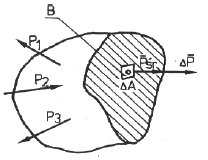
\includegraphics[width=5cm]{Zdjecia/2/potato}
\caption{Ciało pod wpływem sił zewnętrznych \cite{bartek_wolny}}
\label{fig:potato}
\end{figure}

Stana naprężenia w punkcie B oznacza ogół naprężeń, które otrzymamy dla wszystkich możliwych przekrojów ciała przez ten punkt.
W przypadku trójwymiarowego stanu naprężenia, dla każdego przekroju wektor naprężenia będzie miał inny kierunek. Stan naprężenia można opisać przy pomocy tensora naprężeń, dla układu kartezjańskiego danego wzorem:


\begin{gather}
	\sigma=\begin{bmatrix} 
	  \sigma_{xx}    & \tau_{xy} & \tau_{xz} \\ 
	  \tau_{yx} & \sigma_{yy} & \tau_{yz} \\
	  \tau_{zx} & \tau_{zy} & \sigma_{zz} 
	\end{bmatrix}
\end{gather}

gdzie

\begin{eqwhere}[2cm]
        \item[$\sigma_{ii}$] naprężenie normalne, i=(x, y, z)
        \item[$\tau_{ij}$] naprężenie styczne, i,j=(x, y, z), \( i \neq j, \tau_{ij}=\tau_{ji}\)
\end{eqwhere}

\subsection{Odkształcenie i prawko Hooke'a}
\label{sec:odksztalcenie_i_prawo_hookea}

	Pod wpływem naprężeń ciało sprężyste ulega odkształceniu. Możemy wyróżnić odkształcenia liniowe \( \varepsilon_i \) oraz odkształcenia postaciowe \( \gamma_{ij} \). Najprostszym przypadkiem odkształcenia liniowego jest rozciąganie pręta. Poniżej znajduje się rysunek pręta rozciąganego siłą P. 

\begin{figure}[h]
\centering
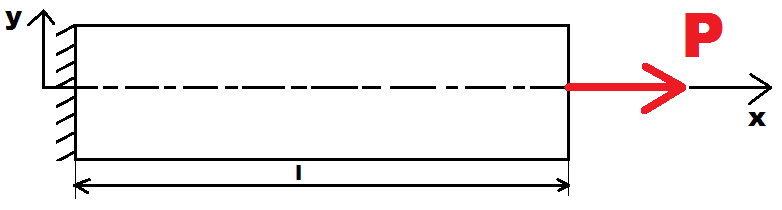
\includegraphics[width=10cm]{Zdjecia/2/rozciaganie}
\caption{Rozciąganie pręta}
\label{fig:rozciaganie}
\end{figure}

	W takim przypadku odkształceniem wzdłużnym będziemy nazywać stosunek wydłużenia pręta do jego początkowej długości:

\begin{equation}
\varepsilon_x=\frac{\Delta l}{l}.
\end{equation}
	
	Odkształceniem poprzecznym(postaciowym) nazywać będziemy stosunek zmiany średnicy przekroju do jego początkowej średnicy:

\begin{equation}
\varepsilon_y=\frac{\Delta d}{d}.
\end{equation}

	Odkształcenia te związane są zależnością:

\begin{equation}
\varepsilon_x=-\nu \varepsilon_y
\end{equation}
gdzie
\begin{eqwhere}[2cm]
        \item[$\nu$] współczynnik Poissona.
\end{eqwhere}

	Współczynnik Poissona jest wielkością bezwymiarową. Określa on sposób w jaki odkształca się ciało i przyjmuje wartości z przedziału [-1, 1]. Dla popularnych w mechanice stopów metali przyjmuje zwykle wartości z przedziału [0.2 , 0.4]. Wartości ujemne przyjmuje dla tak zwanych materiałów odwrotnych, które pod wpływem naprężenia zwiększają swoją objętość.

	Dla przypadku prostego rozciągania zachodzi jeszcze jedna zależność. Opisuje ona związek pomiędzy naprężeniem i odkształceniem i nazywana jest prawem Hooke'a.

\begin{equation}
\sigma=E\varepsilon
\end{equation}
gdzie
\begin{eqwhere}[2cm]
        \item[$E$] moduł Younga.
\end{eqwhere}

	Moduł Younga określa zależność odkształcenia liniowego i przyłożonego naprężenia. Jednostką moduły Younga jest paskal, a wartości podaje się w gigapasklach (GPa). Wartości dla stali wynoszą około 200 GPa, a dla aluminium około 70 GPa.

	W przypadku trójwymiarowego rozkładu okształceń stosuje się zapis tensorowy. Tensor odkształcenia znajduje się poniżej:
\begin{gather}
	\varepsilon=\begin{bmatrix} 
	  \varepsilon_{xx}    & \gamma_{xy} & \gamma_{xz} \\ 
	  \gamma_{yx} & \varepsilon_{yy} & \gamma_{yz} \\
	  \gamma_{zx} & \gamma_{zy} & \varepsilon_{zz} 
	\end{bmatrix}
\end{gather}

%\[
%	\textbf{$\varepsilon$}=\begin{bmatrix} 
%	  \varepsilon_{xx}    & \gamma_{xy} & \gamma_{xz} \\ 
%	  \gamma_{yx} & \varepsilon_{yy} & \gamma_{yz} \\
%	  \gamma_{zx} & \gamma_{zy} & \varepsilon_{zz} 
%	\end{bmatrix}
%\]

gdzie

\begin{eqwhere}[2cm]
        \item[$\varepsilon_{ii}$] odkształcenie liniowe, i=(x, y, z)
        \item[$\gamma_{ij}$] odkształcenie postaciowe, i,j=(x, y, z), \( i \neq j, \tau_{ij}=\tau_{ji}\)
\end{eqwhere}

Dla takiego przypadku prawo Hooke'a przybiera bardziej skomplikowaną postać:

\begin{equation}
\varepsilon_xx=\frac{1}{E}(\sigma_xx-\nu(\sigma_yy+\sigma_zz)), \gamma_{xy}=\frac{\tau_{xy}}{G}
\end{equation}
\begin{equation}
\varepsilon_yy=\frac{1}{E}(\sigma_yy-\nu(\sigma_xx+\sigma_zz)), \gamma_{xz}=\frac{\tau_{xz}}{G}
\end{equation}
\begin{equation}
\varepsilon_zz=\frac{1}{E}(\sigma_zz-\nu(\sigma_xx+\sigma_yy)), \gamma_{yz}=\frac{\tau_{yz}}{G}
\end{equation}

\begin{eqwhere}[2cm]
        \item[$G$] moduł Kirchoffa
\end{eqwhere}

	Moduł Kirchoffa opisuje zależność odkształcenia postaciowego od naprężenia stycznego występującego w materiale. Jednostką tego współczynnika jest paskal, a typowymi wartościami są dla stali 80 Gpa, dla aluminium 25,5 GPa.

	Opisane wcześniej stałe materiałowe są powiązane równaniem:
\begin{equation}
E=2G(\nu+1)
\end{equation}

%\begin{equation}
%c_L=\sqrt{\frac{\lambda+2\mu}{\rho}}
%\end{equation}
%gdzie
%\begin{eqwhere}[2cm]
%        \item[$c_L$] prędkość fali podłużnej
%        \item[$\lambda, \mu$] stałe Lam\'{e}go
%        \item[$\rho$] gęstość ośrodka
%\end{eqwhere}
%
%\begin{figure}[h]
%\centering
%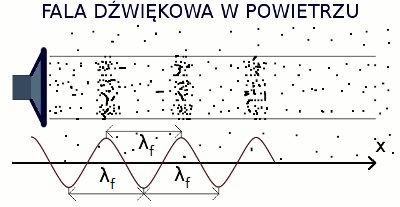
\includegraphics[width=10cm]{Zdjecia/2/fala_podluzna}
%\caption{Przykład fali podłużnej}
%\label{fig:fala_podluzna}
%\end{figure}
%
%
%
%\begin{figure}[h]
%        \centering
%        \begin{subfigure}{0.35\textwidth}
%                \centering
%	     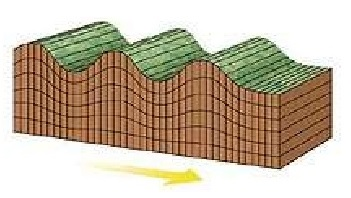
\includegraphics[width=5cm]{Zdjecia/2/fala_rayleigha}
%                \subcaption{\label{subfigure_a}}
%        \end{subfigure}
%        \begin{subfigure}{0.35\textwidth}
%                \centering
%	     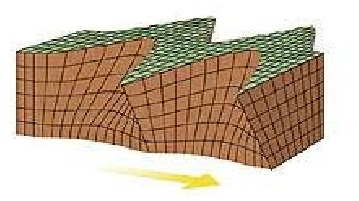
\includegraphics[width=5cm]{Zdjecia/2/fala_lova}
%                \subcaption{\label{subfigure_b}}
%        \end{subfigure}
%        \label{fig:subcaption_example}
%        \caption{Fale powierzchniowe: \protect\subref{subfigure_a} fala Rayleigha, \protect\subref{subfigure_b} fala L\"{o}va}
%\end{figure}

























\section{Rodzaje fal sprężystych}
\label{sec:rodzaje_fal_sprezystych}

Fale można podzielić ze względu na sposób w jaki propagują w materiale. Mogą to być fale podłużne lub poprzeczne. Fale takie propagują jeśli długość fali jest mniejsza lub bliska wymiarom ośrodka. Fale o długości przekraczającej wyraźnie przynajmniej jeden z wymiarów falowodu nazywamy falami prowadzonymi i mają one zupełnie inne własności. Do takich fal możemy zaliczyć np. fale Lamba. Fala Rayleigha z kolei propagują na powierzchniach, stąd ośrodek musi być ograniczony przynajmniej jedną płaszczyzną.

\subsection{Fale podłużne}

Fale podłużne to fale, w których kierunek propagacji jest równoległy z kierunkiem drgania cząstek. Tego typu fale mogą rozchodzić się w każdym ośrodku materialnym. Przykładem fali podłużnej jest fala dźwiękowa rozchodząca się w powietrzu, pokazana na Rys.2.1. Prędkoś fali podłużnej w nieograniczonym ośrodku zależy od parametrów materiałowych ośrodka i dana jest wzorem:

\begin{equation}
c_L=\sqrt{\frac{\lambda+2\mu}{\rho}}
\end{equation}
gdzie
\begin{eqwhere}[2cm]
        \item[$c_L$] prędkość fali podłużnej
        \item[$\lambda, \mu$] stałe Lam\'{e}go
        \item[$\rho$] gęstość ośrodka
\end{eqwhere}

\begin{figure}[h]
\centering
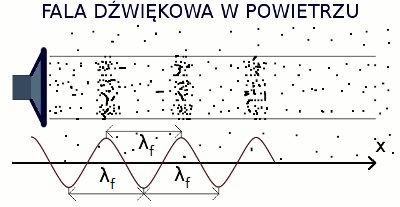
\includegraphics[width=10cm]{Zdjecia/2/fala_podluzna}
\caption{Przykład fali podłużnej}
\label{fig:fala_podluzna}
\end{figure}

Długością fali \( \lambda_f \) nazywamy odległoś między dwoma maksimami (lub minimami), które oznaczają maksymalne zagęszczenie (rozrzedzenie) cząstek w materiale.

\subsection{Fale poprzeczne}

Fale poprzeczne propagują w kierunku prostopadłum do kierunku drgań cząstek. Przykładami takich fal są fale elektromagnetyczne, fale propagacji naprężeń w materiale stałym, czy fala na zamocowanym jednostronnie sznurze, pokazana na Rys.2.2. Prędkoś fali poprzecznej w nieograniczonym ośrodku wyraża się wzorem:

\begin{equation}
c_T=\sqrt{\frac{\mu}{\rho}}
\end{equation}
gdzie
\begin{eqwhere}[2cm]
        \item[$c_T$] prędkość fali poprzecznej
        \item[$\mu$] stała Lam\'{e}go
        \item[$\rho$] gęstość ośrodka
\end{eqwhere}

\begin{figure}[h]
\centering
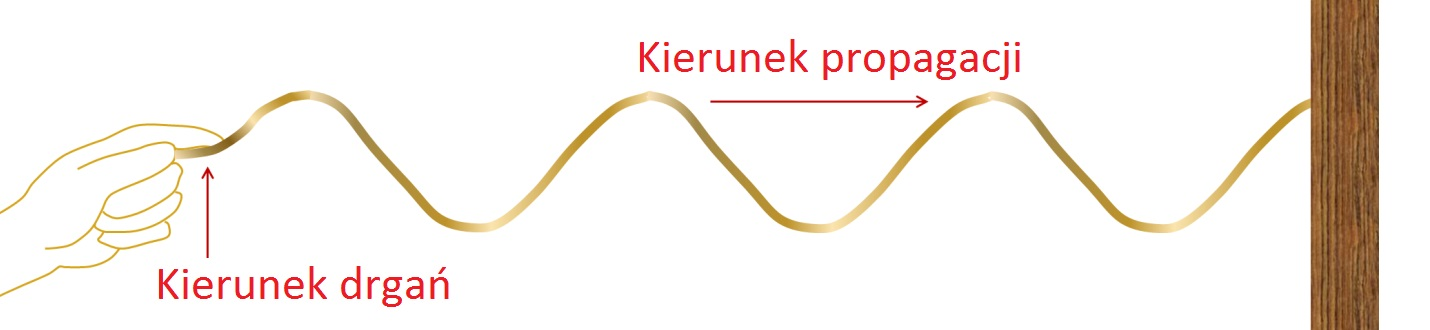
\includegraphics[width=10cm]{Zdjecia/2/fala_poprzeczna}
\caption{Przykład fali poprzecznej}
\label{fig:fala_poprzeczna}
\end{figure}

\subsection{Fale Rayleigha i L\"{o}va}

Opisane wcześniej fale propagują w nieograniczonych mediach. Fale Rayleigha oraz L\"{o}va są falami propagującymi w obszarze powierzchni ciał stałych. Dla fal Rayleigha drgania cząstek odbywają się równolegle oraz prostopadle do kierunku rozchodzenia się fali, zataczając elipsy. Kierunek prostopadły jest normalny do płaszczyzny, na której fala propaguje. Prędkoś fal Rayleigha dla metalu można wyrazić za pomocą współczynnik Poissona i prędkości fal poprzecznych:

\begin{equation}
c_R=\frac{0.87+1.12\cdot\nu}{1+\nu}\cdot c_T
\end{equation}
gdzie
\begin{eqwhere}[2cm]
        \item[$c_R$] prędkość fali Rayleigha
        \item[$c_T$] prędkość fali poprzecznej
        \item[$\nu$] współczynnik Poissona
\end{eqwhere}

Fale L\"{o}va to fale, w których drgania zachodzą w kierunku prostopadłym do kierunku, ale równolegle do płaszczyzny propagacji. Takie fale są wykorzystywane przy badaniu układów wielowarstwowych. Są silnie dyspersyjne, co oznacza że ich prędkość jest funkcją częstotliwości.

\begin{figure}[h]
        \centering
        \begin{subfigure}{0.35\textwidth}
                \centering
	     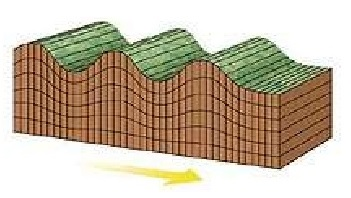
\includegraphics[width=5cm]{Zdjecia/2/fala_rayleigha}
                \subcaption{\label{subfigure_a}}
        \end{subfigure}
        \begin{subfigure}{0.35\textwidth}
                \centering
	     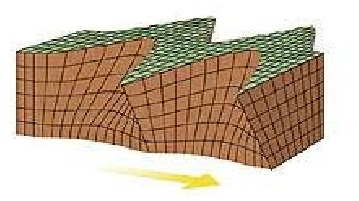
\includegraphics[width=5cm]{Zdjecia/2/fala_lova}
                \subcaption{\label{subfigure_b}}
        \end{subfigure}
        \label{fig:subcaption_example}
        \caption{Fale powierzchniowe: \protect\subref{subfigure_a} fala Rayleigha, \protect\subref{subfigure_b} fala L\"{o}va}
\end{figure}

\subsection{Fale Lamba}

Ważnym typem fal, z racji na szerokie zastosowanie, są fale Lamba. Propagują one na cienkościennych elementach jak płyty, czy rury. Tego typu fale powstają na skutek złożenia dwóch fal Rayleigha, propagujących na płaszczyznach po obu stronach obiektu. Fale Lamba można podzielić na fale symetryczne, kiedy obie fale składowe propagują w tej samej fazie i asntysymetryczne kiedy propagują w innych fazach. Prędkość fal Lamba zależna jest od częstotliwości, ze względu na dyspersyjny charakter.

\begin{figure}[h]
\centering
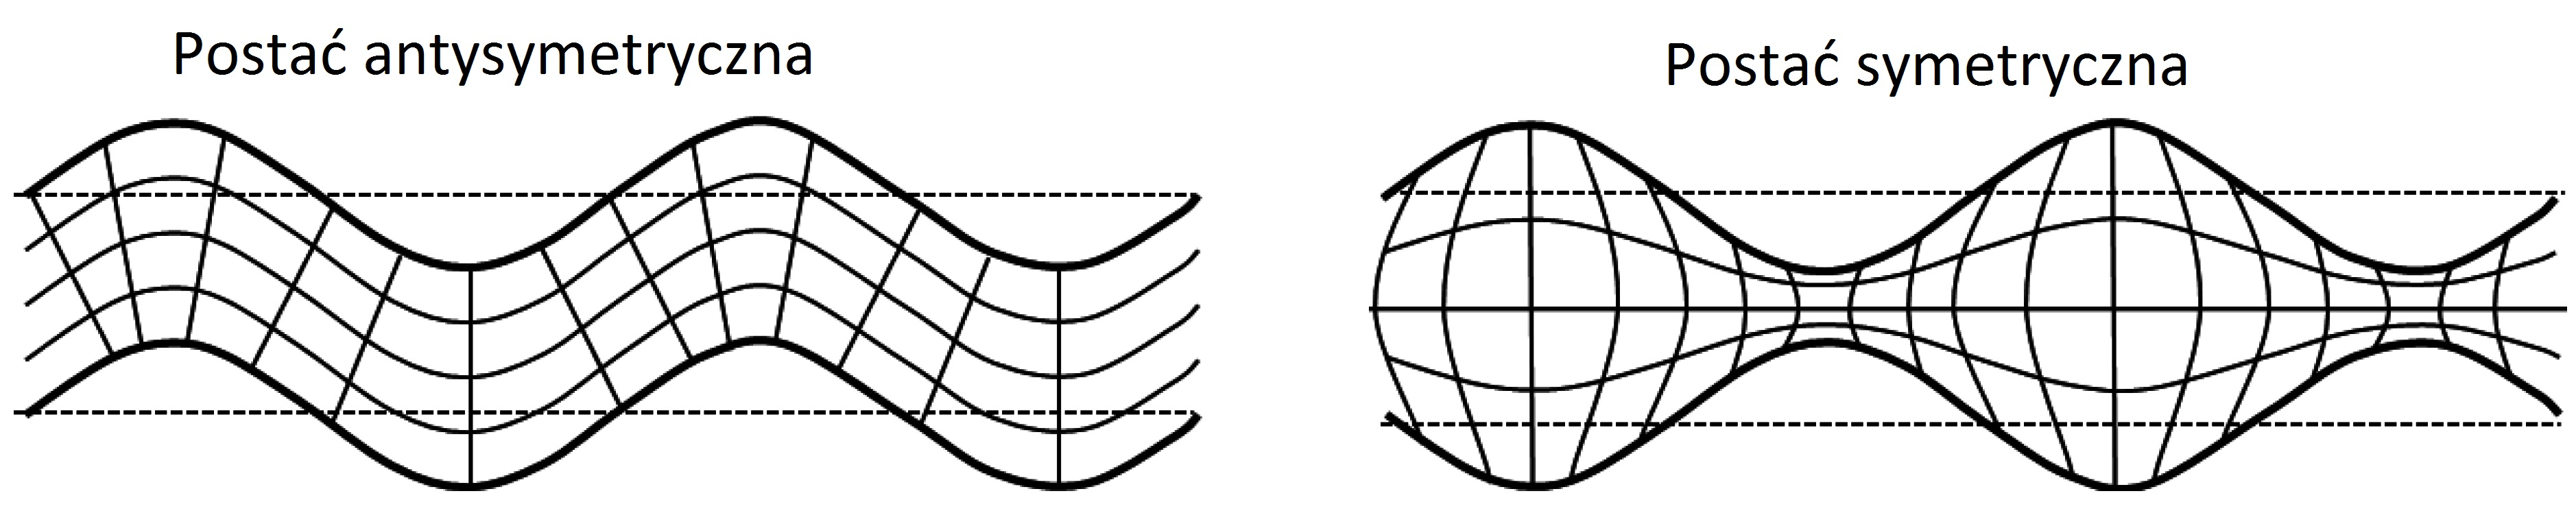
\includegraphics[width=14cm]{Zdjecia/2/fala_lamba}
\caption{Fale Lamba}
\label{fig:fala_lamba}
\end{figure}

%---------------------------------------------------------------------------
























\section{Zjawisko dyspersji}
\label{sec:rodzaje_fal_sprezystych}

Dyspersja jest zjawiskiem zależności prędkości propagacji fali od jej częstotliwości. Częstotliwością fali nazywamy liczbę pełnych przebiegów (np. od maximum do maximum) w jednostce czasu. Jednostką częstotliwości jest herc (Hz). Wielkością równie często używaną jest częstość kołowa dana wzorem \( \omega = 2\pi f \). Jej jednostką jest radian na sekundę [rad/s]. Odpowiednikiem tego parametru dla wymiarów geometrycznych jest liczba falowa. Określa ona jak wiele długości fali zawiera fala w jednostce odległości. Jednostką liczby falowej jest radian na metr [rad/m].

\begin{figure}[h]
\centering
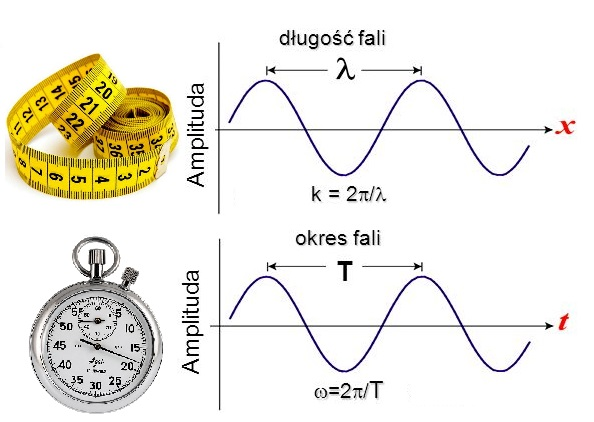
\includegraphics[width=10cm]{Zdjecia/2/czestotliwosc1}
\caption{Częstotliwość \( \omega \) i liczba falowa k}
\label{fig:czestotliwosc_i_liczba_falowa}
\end{figure}


Kiedy mówimy o krzywych dyspersji, możemy mieć na myśli zależności liczby falowej od częstotliwości, prędkości fazowej od częstotliwości lub prędkości grupowej od częstotliwości. Na rysunku \ref{fig:krzywe_k_od_omega} znajdują się przykładowe charakterystyki k(\(\omega\)) postaci fal Lamba dla aluminiowej płyty o grubości 1mm.

\begin{figure}[h]
\centering
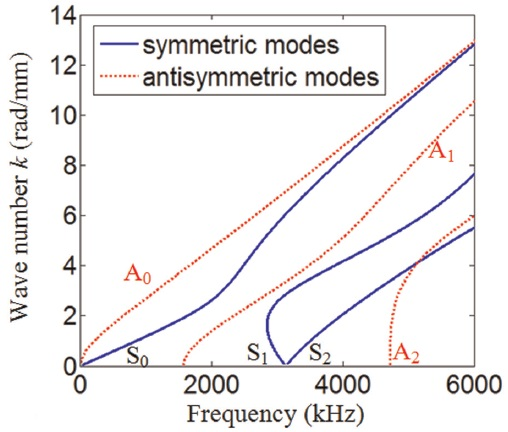
\includegraphics[width=10cm]{Zdjecia/2/char_fazowa}
\caption{Krzywe k(\(\omega\)) \cite{bartek_tian}}
\label{fig:krzywe_k_od_omega}
\end{figure}

Na wykresach widać jedną rzecz, ważną dla zastosowań fal prowadzonych - są one multimodalne. Z wykresów wynika, że w najkorzystniejszym do analizy przypadku propagują dwa mody, jeden symetryczny i jeden antysymetryczny. Wraz ze wzrostem częstotliwości propagującej fali pojawiają się dodatkowe jej postaci, co znacznie utrudnia analizę danych z przebiegów. Jednym ze sposobów ograniczania liczby modów, jest wprowadzanie wymuszeń o niskich częstotliwościach.

\subsection{Prędkość fazowa i grupowa}

Prędkość fazowa określa jak szybko przemieszcza się punkt fali o stałej fazie. Dla fali sinusoidalnej u(x,t)=sin(kx-\(\omega\)t) można wyznaczyć zależność na prędkość fazową w następujący sposób:

\begin{equation}
kx-\omega t=const \Rightarrow \frac{d(kx-\omega t)}{dt}=0 \Rightarrow k\frac{dx}{dt}-\omega=0
 \Rightarrow \frac{dx}{dt}=\frac{\omega}{k}
\end{equation}

Jak widać dla skończonej wartości \(\omega\) i k dążącego do zera, prędkość fazowa rośnie do nieskończoności. Dla przypadku pierwszych modów, gdzie zarówno k jak i \(\omega\) zmierzają do zera, sytuacja wygląda różnie. Na rysunku \ref{fig:krzywe_vp_od_omega} znajduje się przykładowy wykres zależności prędkości fazowej od iloczynu częstotliwości i grubości materiału dla cienkościennej rury. W przypadku fal prowadzonych dla elementów cienkościennych, często wykreśla się charakterystyki z zaznaczeniem wpływu grubości ściany. Na wykresie widać, że wszystkie mody poza pierwszymi dwoma dążą prawostronnie do nieskończoności. Pozostałe dwa zachowują się odmiennie - jeden wykres dąży do 0 (postać antysymetryczna), a drugi do wartości skończonej (postać symetryczna).

\begin{figure}[h]
\centering
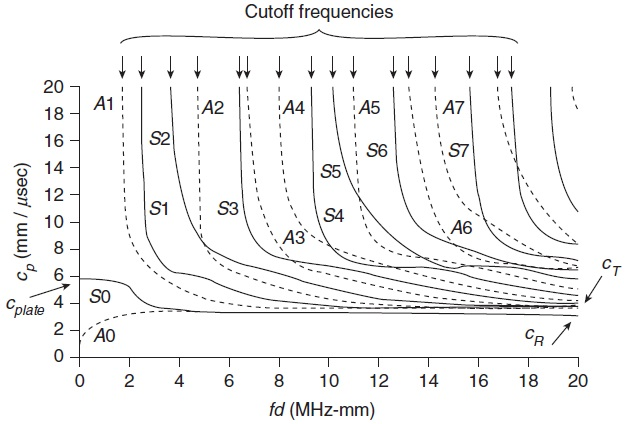
\includegraphics[width=10cm]{Zdjecia/2/char_predkosc_fazowa}
\caption{Krzywe \(V_p(\omega\)) \cite{bartek_rose}}
\label{fig:krzywe_vp_od_omega}
\end{figure}

Jeśli fala składa się z więcej niż jednej składowej sinusoidalnej, które mają różne prędkości, należy określić jeszcze prędkość grupową.  Prędkość każdej z pojedynczych składowych, będzie jej prędkością fazową. Prędkość grupowa dotyczy sygnału, złożonego ze wszystkich składowych. Można ją prezentować jako prędkość punktu o zmiennej fazie na wykresie sygnału, np. maximum, jak na rysunku \ref{fig:przykladowy_sygnal}.

\begin{figure}[h]
\centering
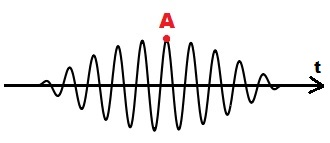
\includegraphics[width=10cm]{Zdjecia/2/predkosc_grupowa_wierzcholek}
\caption{Przykładowy sygnał. Prędkość punktu A jest prędkością grupową}
\label{fig:przykladowy_sygnal}
\end{figure}

Weźmy sygnał złożony z kilku sinusoid o zbliżonej częstości. Fazę każdego sygnału można zapisać jako \( \omega_i t - k_i T + \phi_i \), gdzie \( i\) oznacza numer składowej. Założmy, że fazy tych sygnałów są równe w punkcie x=0, t=0. Wynika stąd, że \( \phi_i \) są niezależne od \( \omega \). Punkt x=0, t=0 będzie maksimum, ponieważ wszystkie składowe zsumują się w tym punkcie. Aby znaleźć kolejny punkt z takim maximum, należy określić gdzie fazy po raz kolejny będą sobie równe.  Punkt, w którym to zjawisko zajdzie musi być niezależny od \( \omega \), w otoczeniu pewnego \( \omega \). Symbolicznie można to zapisać jako:

\begin{equation}
\frac{d(\omega t - kx - \phi)}{d\omega}=0 \Rightarrow t-\frac{dk}{d\omega}x=0 \Rightarrow \frac{x}{t}=\frac{d\omega}{dk}
\end{equation}

Maximum sygnału będzie więc w każdym punkcie x, t spełniającym powyższą zależność. Prędkość grupowa fali jest więc równa:

\begin{equation}
V_g=\frac{dw}{dk}
\end{equation}

Z samego faktu istnienia takiej zależności nie wynika, że w sygnale znajdzie się jakiś charakterystyczny punkt, propagujący z taką prędkością. Wynika z niej natomiast, że jeśli takowy punkt będzie, to będzie się poruszał z prędkością grupową. Należy jeszcze wspomnieć o wyznaczaniu prędkości grupowej sygnału o składowch, o różnych wartościach \( \omega \). W takim przypadku należy prędkość grupową wyznaczyć dla wartości \(\omega\) sygnału dominującego. Dominujący sygnał można znaleźć przy pomocy przekształecenia Fouriera.

Na rysunku \ref{fig:predkosc_grupow_wykres} znajdują się przykładowe krzywe, przedstawiające prędkość grupową dla fal Lamba, dla cienkościennej płyty aluminiowej.

\begin{figure}[h]
\centering
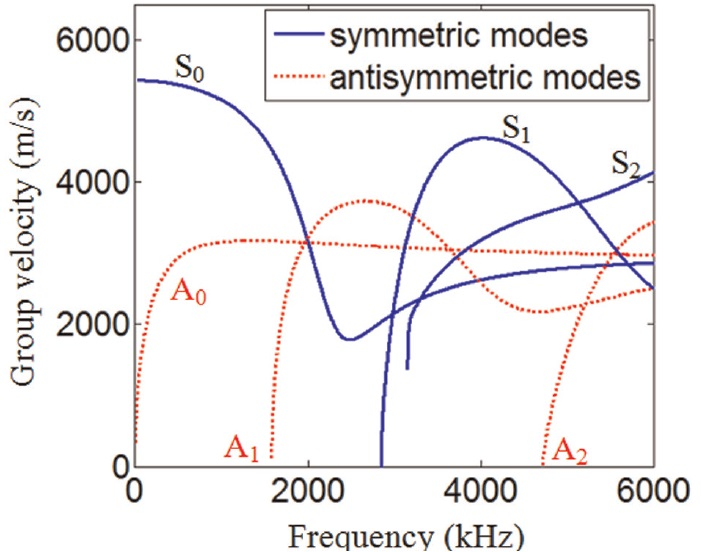
\includegraphics[width=10cm]{Zdjecia/2/predkosc_grupowa_wykres}
\caption{Wykres prędkości grupowej \(V_g(\omega)\) \cite{bartek_tian}}
\label{fig:predkosc_grupow_wykres}
\end{figure}


\subsection{Analityczne wyznaczanie krzywych dyspersji}

Zależności dyspersyjne są trudne, a często niemożliwe do wyznaczenia w sposób analityczny. Dla prostych przypadków rozwiązania analityczne są znane, a kilka z nich jest poniżej opisanych w celu lepszego wyjaśnienia zjawiska dyspersji.
Pierwszym przypadkiem będzie model nieskończenie długiej, napiętej sprężyny, przedstawionej na rysunku \ref{fig:nieskonczenie_krotki_odcinek_sprezyny}.

\begin{figure}[h]
\centering
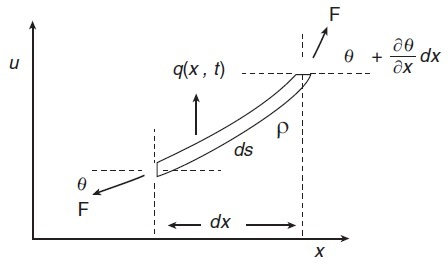
\includegraphics[width=10cm]{Zdjecia/2/dyspersja_analitycznie_sprezyna}
\caption{Nieskończenie krótki odcinek napiętej sprężyny \cite{bartek_rose}}
\label{fig:nieskonczenie_krotki_odcinek_sprezyny}
\end{figure}

Symbole z rysunku oznaczają:

\begin{eqwhere}[2cm]
        \item[$ds$] długość sprężyny
        \item[$\theta$] kąt przyłożenia siły zewnętrznej
        \item[$F$] siły wewnętrzne
        \item[$q$] siła oddziaływania sprężyny na jednostkę długości ugięcia
        \item[$\rho$] masa sprężyny na jednostkę długości.
\end{eqwhere}

Korzystając z drugiej zasady dynamiki Newtona, zapisujemy równanie ruchu układu:

\begin{equation}
-Fsin\theta+Fsin(\theta+\frac{\partial \theta}{\partial x}dx)+qds = \rho ds \frac{\partial^2u}{\partial t^2}.
\end{equation}

Załóżmy dodatkowo, że:

\begin{equation}
ds \approx dx\; ,\; sin\theta=\theta \; i\; \theta = \frac{\partial u}{\partial x}.
\end{equation}

To pozwala uprościć równanie:

\begin{equation}
-F\theta+F(\theta + \frac{\partial \theta}{\partial x}dx)=\rho dx\frac{\partial^2 u}{\partial^2 t}
\end{equation}

\begin{equation}
F\frac{\partial^2 u}{\partial x^2} + q = \rho \frac{\partial^2 u}{\partial^2 t}.
\end{equation}

Jeśli założymy brak siły zewnętrznej, to otrzymujemy proste równanie falowe:

\begin{equation}
\frac{\partial^2 u}{\partial x^2} = \frac{1}{c_0^2} \frac{\partial^2 u}{\partial^2 t},\quad c_0=\sqrt{\frac{F}{\rho}}
\end{equation}

gdzie
\begin{eqwhere}[2cm]
        \item[$c_0$] prędkość fali.
\end{eqwhere}

Przyjmijmy rozwiązanie w postaci:

\begin{equation}
u(x,t)=Ae^{i(kx-\omega t)}.
\end{equation}

Jeśli wstawimy je do równania falowego to otrzymamy zależność dyspersyjną:

\begin{equation}
\omega^2=c_0^2 k^2.
\end{equation}

Jest to przypadek liniowej zależności \( k(\omega)\), a więc dyspersja fali nie zachodzi. W takim przypadku prędkość fazowa, jest równa prędkości grupowej:

\begin{equation}
V_p=\frac{\omega}{k}=\frac{d\omega}{dk}=V_g
\end{equation}

Prosta modyfikacja układu ze sprężyną jak na rysunku \ref{fig:nieskonczenie_krotki_odcinek_sprezyny2}, powoduje skomplikowanie zależności dyspersyjnej.

\begin{figure}[h]
\centering
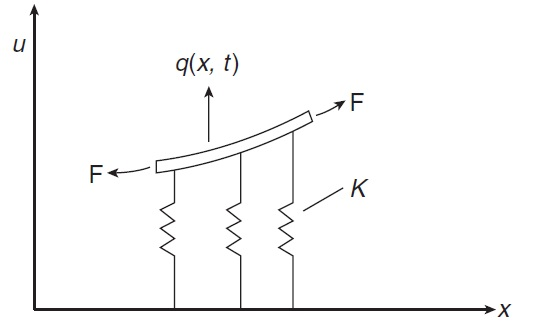
\includegraphics[width=10cm]{Zdjecia/2/dyspersja_analitycznie_sprezyna2}
\caption{Nieskończenie krótki odcinek napiętej sprężyny na sprężystym podłożu \cite{bartek_rose}}
\label{fig:nieskonczenie_krotki_odcinek_sprezyny2}
\end{figure}

Przyjmijmy siłę \(q=-Ku(x,t)\), co prowadzi do równania równowagi:

\begin{equation}
\frac{\partial^2 u}{\partial x^2} - \frac{K}{F}u = \frac{1}{c_0^2} \frac{\partial^2 u}{\partial^2 t}.
\end{equation}

Ponownie załóżmy rozwiązanie w postaci \( u(x,t)=Ae^{i(kx-\omega t)} \) i podstawmy je do równania równowagi. Prowadzi to do zależności:

\begin{equation}
\Big(-k^2-\frac{K}{F}+\frac{w^2}{c_0^2}\Big)e^{i(kx-\omega t)}=0.
\end{equation}

Równanie to jest nazywane równaniem charaktersytycznym (lub dyspersyjnym). Rozwiązaniem jest:

\begin{equation}
-k^2-\frac{K}{F}+\frac{w^2}{c_0^2}=0.
\end{equation}

Zależność \(k(\omega)\) przyjmuje postać:

\begin{equation}
k^2=\frac{w^2}{c_0^2}-\frac{K}{F}.
\end{equation}

Podstawiając \( k=\frac{\omega}{c_p}\), otrzymujemy :

\begin{equation}
c_p = \sqrt{c_0^2\Bigg( \frac{1}{1 - \frac{c_0^2 K}{\omega^2 F} } \Bigg)}.
\end{equation}

Jak widać w takim przypadku prędkość fazowa jest zależna od częstotliwości, a więc będzie zachodzić dyspersja fali.

\vspace{3mm}

Kolejnym problemem wartym wspomnienia, jest problem propagacji fal Lamba w cienkiej, nieskończonej płycie. Płyta wraz z przyjętym układem współrzędnych znajduje się na rysunku \ref{fig:nieskonczona_plyta}.

\begin{figure}[h]
\centering
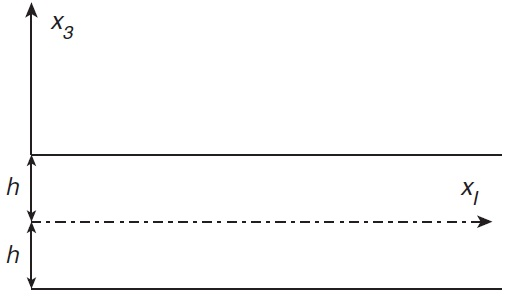
\includegraphics[width=10cm]{Zdjecia/2/dyspersja_analitycznie_plyta}
\caption{Nieskończona płyta \cite{bartek_rose}}
\label{fig:nieskonczona_plyta}
\end{figure}

Jest kilka metod rozwiązania takiego zagadnienia, ale nie są opisane one w tej pracy (metoda potencjałów, metoda fal cząstkowych). Jeśli przyjmiemy zerowe naprężenia na płaszczyznach zewnętrznych jako warunki początkowe, to związki dyspersyjne przyjmują zależności:

\begin{equation}\label{fig:RL1}
\frac{tan(qh)}{tan(ph)}=-\frac{4k^2pq}{(q^2-k^2)^2}
\end{equation}
dla postaci symetryczych oraz

\begin{equation}\label{fig:RL2}
\frac{tan(qh)}{tan(ph)}=-\frac{(q^2-k^2)^2}{4k^2pq}
\end{equation}
dla postaci antysymetrycznych,

gdzie
\begin{equation}
p^2=\frac{\omega^2}{c_L^2} - k^2 \; ,a \; q^2=\frac{\omega^2}{c_L^2}-k^2
\end{equation}

\begin{eqwhere}[2cm]
        \item[$c_T$] prędkość fali poprzecznej
	\item[$c_L$] prędkość fali podłużnej
\end{eqwhere}

Równania \ref{fig:RL1}, \ref{fig:RL2} nazywają się równaniami Rayleigha-Lamba i są nierozwiązywalne w sposób analityczny. Jest to przykład bardziej skomplikowanego modelu, gdzie możliwe jest wyznaczenie związków \(k\) i \(\omega\), ale do wykreślenia krzywych dyspersji konieczne jest zastosowanie metod numerycznych.



\subsection{Numeryczne wyznaczanie krzywych dyspresji}
Pierwszym przypadkiem numerycznego wyznaczania krzywych dyspersji, jest rozwiązanie równań Rayleigha-Lamba przedstawionych w poprzedniej sekcji. Zakładamy, że interesują nas tylko rozwiązania rzeczywiste, które pojawią się jeśli k przyjmie wartości rzeczywiste bądź urojone (w równaniach występuje tylko czynnik \(k^2\)).

Poniżej znajdują się równania Rayleigha-Lamba w postaci ułatwiającej proponowany sposób rozwiązania:

\begin{equation}
\frac{tan(qh)}{q}+\frac{4k^2ptan(ph)}{{q^2-k^2}^2}=0
\end{equation}

\begin{equation}
qtan(qh)+\frac{{(q^2-k^2)}^2tan(ph)}{2k^2p}=0.
\end{equation}

\vspace{5mm}

Rozwiązać równanie możemy według przedstawionego algorytmu.

\begin{enumerate}
  \item Wybierz iloczyn \((\omega h)_0\).
  \item Wybierz początkową estymatę prędkości fazowe \((c_p)_0\) (a pośrednio też \(k\)).
  \item Oblicz znak lewych stron równań R-L.
  \item Wybierz kolejną wartość prędkości fazowej \((c_p)_1 > (c_p)_0\) i policz znaki lewych stron jeszcze raz.
  \item Powtarzaj kroki 3 i 4 aż znaki się zmienią. Oznaczać to bedzie, że pierwiastek równania znajduje się pomiędzy ostatnio wybranymi prędkościami. Załóżmy, że jest to pomiędzy \( (c_p)_n \) i \( (c_p)_{n+1} \).
  \item Wykorzystaj jakiś algorytm iteraycjny do znalezienia pierwiastka \(c_p\) z odpowiednią dokładnością.
   \item Po znalezienu pierwiastka, kontynuuj wyszukiwnie kolejnych pierwiastków dla założonego \( (\omega h)_0 \), powtarzając kroki 2-6.
  \item Wybierz kolejną wartość \( \omega h \) i wykonaj dla niej kroki 2-7.
\end{enumerate}

\vspace{5mm}

W ten sposób łatwo wyznaczyć krzywe dyspersji, ale należy zaznaczyć, że równania dyspersyjne zostały obliczone analitycznie dla konkretnego przypadku struktury, jaką jest płyta. Metody numeryczne ograniczają się w tym przypadku do rozwiązania wyznaczonych równań. Możliwość ogólniejszego podejścia do badań numerycznych, dla szerokiego wachlarza struktur daje metoda elementów skończonych.

Metoda ta daje możliwości dokładnego przewidzenia odpowiedzi dynamicznych, dla złożonych układów mechanicznych. Jeśli założymy przypadek małych odkształceń, to problem można zapisać w postaci równania różniczkowego:

\begin{equation} \label{eq:MES1}
M\ddot u + Ku = f^{ext}
\end{equation}

gdzie
\begin{eqwhere}[2cm]
        \item[$M$] macierz mas układu
        \item[$K$] macierz sztywności układu 
        \item[$u$] przemieszczenia punktów układu
        \item[$f^{ext}$] wektor sił zewnętrznych
\end{eqwhere}

Sposobem wyznaczenia krzywych dyspersji z tak określonego układu, może być rozwiązanie równania tj. znalezienie pola przemieszczeń dla wszystkich węzłów w dyskretnych chwilach czasowych, a następnie obliczenie wielowymiarowego przekształcenia Fouriera otrzymanego sygnału.

Równanie można rozwiązać na przykład z wykorzystaniem centralnej formuły różnicowej dla \( \ddot u\):

\begin{equation}
\ddot x = \frac{u^{t+1} - 2u^t + u^{t-1}}{\Delta t^2}.
\end{equation}

Po podstawienu otrzymujemy zależność:

\begin{equation}
\frac{1}{\Delta t^2}M(u^{t-1}-2u^t+u^{t-1}) + Ku^t = f^t
\end{equation}

\begin{equation}
u^{t+1}=\Delta t^2 M^{-1}(f^t -Ku^t)+2u^t-u^{t-1}
\end{equation}

gdzie \( t \) oznacza obecną chwilę czasową, a \( t+1 \) chwilę kolejną.
Operacja odwracania macierzy mas jest kosztowna obliczeniowo. Można przyśpieszyć obliczenia przez zastosowanie skupionej macierzy mas (wyrazy niezerowe tylko na głownej diagonali).

Jeśli interesuje nas propagacja tylko w jednym kierunku, to dla obliczonego sygnału \( u[m, n] \) (m - liczba kroków czasowych \(\Delta t \) , n - liczba kroków geometrycznych \(\Delta x\) w kierunku x) przekształcenie Fouriera można obliczyć według wzoru:

\begin{equation} \label{eq:fourier_2d}
U[p, q] = \sum_{k=0}^{m-1} \sum_{l=0}^{n-1} u[k, l]e^{-i2\pi (-p \frac{k}{m} + q\frac{l}{n})}
\end{equation}

Mając dyskretną postać przekształcenia Fouriera można wykreślić krzywe dyspersji, wyznaczając dla każdej próbki wartość czętotliwości i liczby falowej. Można to zrobić wiedząc, że częstość zawiera się w przedziale \([0, \frac{1}{2\Delta t}2\pi]\), a liczba falowa \([0, \frac{1}{2\Delta x}2\pi]\). Przykładowe krzywe przedstawione są na rysunku \ref{fig:krzywe_dyspersji_tian1}.

\vspace{5mm}

\begin{figure}[h]
\centering
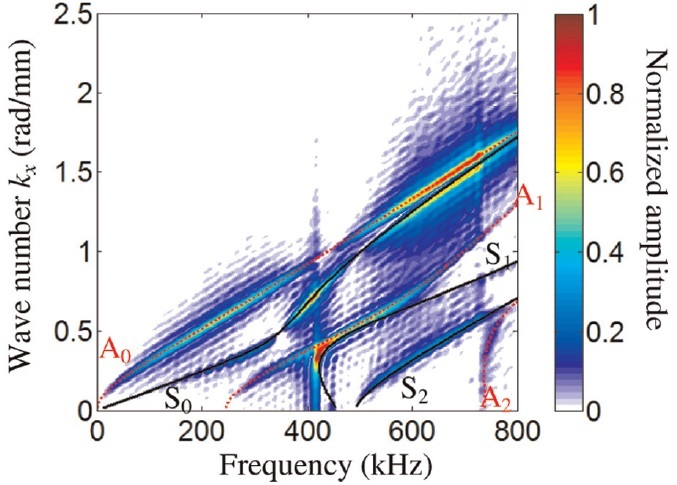
\includegraphics[width=10cm]{Zdjecia/2/dyspersja_tian1}
\caption{Krzywe dyspersji wyznaczone przy pomocy dwuwymiarowego DFT}
\label{fig:krzywe_dyspersji_tian1}
\end{figure}

Innym sposobem wyznaczania krzywych dyspersji z pomocą modelu MES, jest symulacja układu dla wymuszeń harmonicznych o ustalonych częstotliwościach, w których chcemu wyznaczyć krzywe. Jako przyład rozpatrzmy jednorodny pręt. Dla przypadku pręta wymuszanego na jednej płaszczyźnie przekroju, dane należy zebrać przed odbiciem fali od swobodnego końca pręta, tak aby sygnał propagował tylko w jednym kierunku. W liniach równoległych do osi, obliczamy pola prędkości przemieszczenia punktów. Może to być też pole przemieszczeń lub naprężeń, ale pole prędkości jest stosunkowo łatwe do wyznaczenia.
Znając już prędkości dla wszystkich punktów w jednej lini, w chwili t, możemy wyznaczyć widmo otrzymanego sygnału. Następnie z widma sygnału odczytujemy liczby falowe, dla których powstały widoczne piki. Pik dla największej liczby falowej dotyczy pierwszego modu, a każdy kolejny, z coraz mniejszymi liczbami falowymi, modów kolejnych.

Pole prędkości można wyznaczyć na podstawie różnycowych formuł centralnych \ref{eq:MES2} oraz \ref{eq:MES3}.

\begin{equation} \label{eq:MES2}
\dot u^{t+1} = \dot u^n + \frac{\Delta t}{2}(\ddot u^n + \ddot u^{n+1})
\end{equation}

\begin{equation} \label{eq:MES3}
u^{n+1} = u^n + \Delta t(\dot u^n + \frac{\Delta t}{2}\ddot u^n)
\end{equation}

Załóżmy, że znamy pełne rozwiązanie w chwili t. Przemieszczenie w chwili t+1 możemy więc obliczyć z zależności \ref{eq:MES3}. Następnie podstawiamy wynik do równania \ref{eq:MES1} i obliczamy przyspeszenie w chwili t+1. Ostatecznie korzystając z formuły \ref{eq:MES2} możemy wyznaczyć prędkość w chwili t+1.

Przykładowe widmo, z którego możemy odczytać liczby falowe czterech modów znajduje się na rysnuku \ref{fig:widmo_wymuszenie1}. Jak widać nie wszystkie liczby falowe da się wykryć przy pomocy danych z jednej lini, więc niezbędne jest prowadzenie obliczeń dla kilku różnych linii.

\begin{figure}[h]
\centering
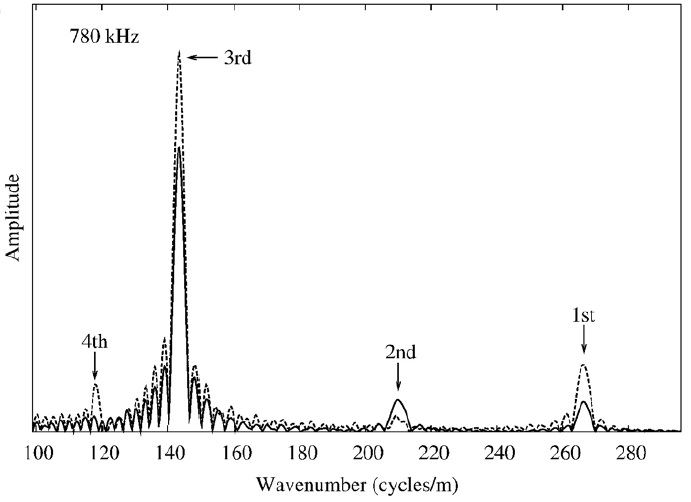
\includegraphics[width=10cm]{Zdjecia/2/widmo_wymuszenia_waskopasmowe}
\caption{Widmo sygnału prędkości na liniach równoległych do osi pręta}
\label{fig:widmo_wymuszenie1}
\end{figure}

Wadą tego sposobu jest konieczność prowadzenia obliczeń dla każdej częstotliwości, dla jakiej chcemy mieć punkty krzywych dyspersji. Jedne przebieg daję nam tylko jeden punkt na każdej krzywej. Fakt prowadzenia obliczeń tylko w liniach równoległych do osi pręta, ogranicza dodatkow obszar propagujących fal do fal podłużnych.

\vspace{3mm}

Sposobem zmniejszenia liczby symulacji jakie trzeba przeprowadzić jest symulacja z wymuszeniem szerokopasmowym. Pozwala to na uzyskanie informacji o krzywych dyspersji, dla częstotliwości zawierających się w wymuszającym sygnale. Pojawia się jednak kilka dodatkowych kroków jakie trzeba wykonać, aby uzyskać liczby falowe modów dla poszczególnych częstotliwości.

Aby uzyskać dane do wykreślenia krzywych dyspersji, należy obliczyć przestrzenny rozkład prędkości na liniach równoległych do osi dla wszystkich częstotliwości. W tym celu trzeba wykonać następujące czynności.

\begin{enumerate}
  \item Wyznaczyć odpowiedzi czasowe dla każdego punktu na interesującej nas lini równoległej do osi pręta.
  \item Obliczyć transformaty Fouriera tych sygnałów
  \item Z widma sygnału w każdym punkcie pobrać informacje o amplitudzie dla kolejnych częstotliwości. Na tej podstawie odtworzyć amplitudowy przebieg sygnału na całej lini dla każdej interesującej nas częstotliwości.
  \item Dla obliczonych w pkt. 3 przebiegów, obliczyć transformatę Fouriera i z wykresu odczytać wartości liczby falowej, dla wybranych częstotliwości.
\end{enumerate}

Rysunki \ref{fig:szer_odp_czasowe} oraz \ref{fig:szer_odp_przestrzenne} przedstawiają kolejne kroki postępowania, dla odpowiedzi na wymuszenie krokiem jednostkowym preta zbudowanego z 1601 węzłów na długości jednej lini. 

\begin{figure}[h]
\centering
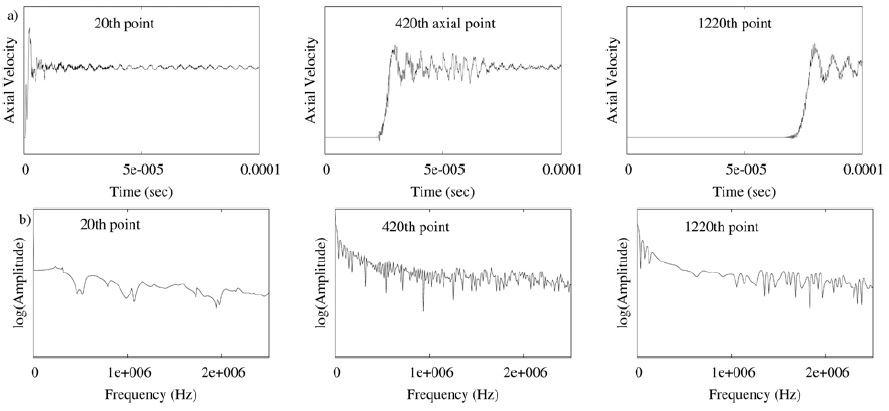
\includegraphics[width=12cm]{Zdjecia/2/widmo_wymuszenia_szerokopasmowe1}
\caption{a) Odpowiedzi na szerokopasmowe wymuszenie w wybranych punktach jednej lini b) Przekształcenia Fouriera odpowiedzi czasowych}
\label{fig:szer_odp_czasowe}
\end{figure}

\begin{figure}[h]
\centering
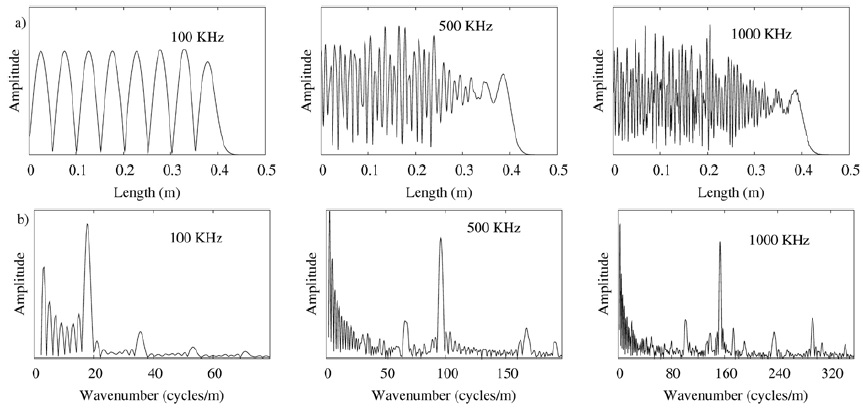
\includegraphics[width=12cm]{Zdjecia/2/widmo_wymuszenia_szerokopasmowe2}
\caption{a) Odtworzony sygnał apmlitudowy na długości pręta w jednej lini b) Przekształcenie Fouriera odtworzonych sygnałów}
\label{fig:szer_odp_przestrzenne}
\end{figure}

\vspace{3mm}

Ostatnia przedstawiona tutaj metoda skupia się, na rozwiązaniu zagadnienia własnego modelu wyznaczonego z pomocą MES. Tym razem zakładać będziemy wybraną liczbę falową i dla niej obliczać częstości poszczególnych modów. 
Po raz kolejny za przykład weźmy pręt. Pręt dzielimy na komórki, które będą się składać z kolejnych płaszczyzn, na których znajdują się węzły. Znając odległość płaszczyzn i wybierając liczbę falową, możemy okrelić przesunięcie fazowe fali pomiędzy płaszczyznami. Sytuacja przedstawiona jest na rysunku \ref{fig:komorki_preta}.


\begin{figure}[h]
\centering
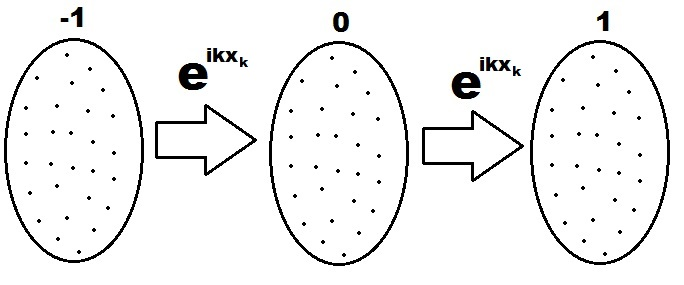
\includegraphics[width=10cm]{Zdjecia/2/metoda_numeryczna3}
\caption{Kolejne komórki pręta}
\label{fig:komorki_preta}
\end{figure}

W liniowych systemach do opisu popagacji fali wystarcza jedna komórka i siły wewnętrzne pochodzące od komórek sąsiednich. W przypadku braku sił zewnętrznych i przy założeniu skupionej macierzy mas, równanie układu można zapisać w postaci \ref{eq:MES4}. Rysunek \ref{fig:komorki_preta_sztywnosc} przedstawia sposób wyznaczania macierzy sztywności dla komórki środkowej, z uwzględnieniem zależności z komórkami sąsiednimi.

\begin{equation} \label{eq:MES4}
M_0\ddot x_0 + \sum_{p=-1}^1 K_p x_p = 0
\end{equation}

\begin{figure}[h]
\centering
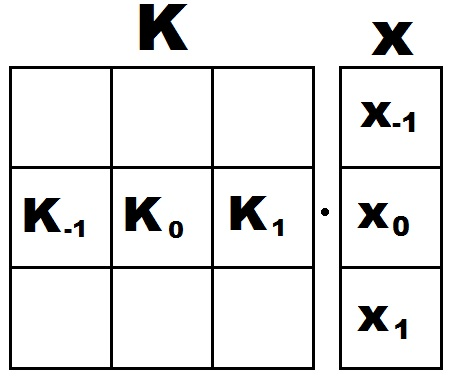
\includegraphics[width=8cm]{Zdjecia/2/metoda_numeryczna3_sztywnosc}
\caption{Wyznaczanie macierzy sztywności środkowej komórki z uwzględnieniem zależności z komórkami sąsiednimi}
\label{fig:komorki_preta_sztywnosc}
\end{figure}

Uwzględniając wszystkie informacje równanie układu można zapisać jako \ref{eq:MES5}. Podstawiając dodatkowo zależności \( \ddot x = x \omega^2 \), \( M_{sys} = M_0 \) oraz \( K_{sys} = K_{-1} e^{-ikx_k} + K_0 + K_1 e^{ikx_k} \) otrzymujemy równanie \ref{eq:MES6}.

\begin{equation} \label{eq:MES5}
M_0\ddot x_0 + K_{-1} x_0 e^{-ikx_k} + K_0 x_0 + K_1 x_0 e^{ikx_k} = 0
\end{equation}

\begin{equation} \label{eq:MES6}
 (M_{sys}\omega^2 + K_{sys})x_0 = 0
\end{equation}

Ostatecznie rozwiązując zagadnienie własne dla pary macierzy \( M_{sys} \) i \( K_{sys} \) otrzymujemy kwadraty częstości własnych układu dla założonego \( k \). Każda z częstości należy do jednego modu krzywych dyspersji.

Wadami tej metody są konieczność prowadzenia obliczeń dla każdej liczby falowej, którą chcemy uwzględnić w wynikach, oraz brak dokładnej informacji, która częstość własna należy do której postaci fali.

Dużą zaletą z kolei jest fakt, że wyznaczamy jedną metodą krzywe dyspersji dla fal podłużnych i poprzecznych.

Przykładowe krzywe dyspersji uzyskane w ten sposób przedstawia rysunek \ref{fig:przykladowe_krzywe}.

\begin{figure}[h]
\centering
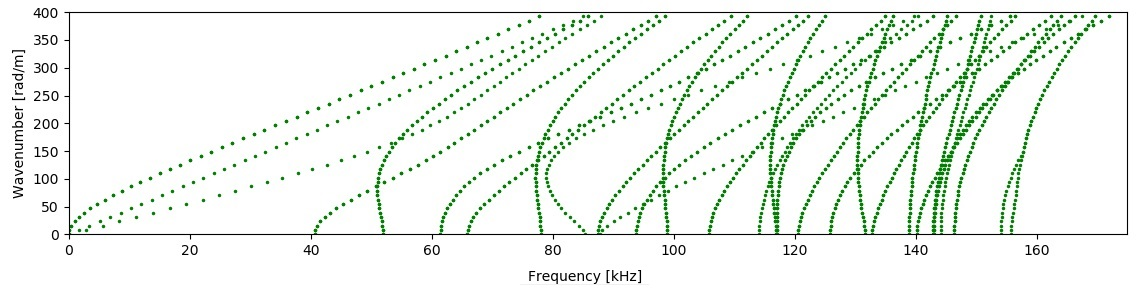
\includegraphics[width=14cm]{Zdjecia/2/przykladowe_krzywe}
\caption{Krzywe uzyskane przez wielokrotne rozwiązanie zagadnienia własnego pręta}
\label{fig:przykladowe_krzywe}
\end{figure}



\subsection{Eksperymentalne wyznaczanie krzywych dyspersji}

Eksperymentalne badania fal prowadzonych przeprowadza się wzbudzając odpowiednio obiekt, a następnie zbiera się dane o powstałej fali w innych punktach konstrukcji lub w tym samym punkcie po odbiciu fali. Zebrane dane analizuje się za pomocą algorytmów, w których duże znaczenie ma przekształcenie Fouriera.

Jako wzbudniki fal prowadzonych często stosowane są przetworniki piezoelektryczne (na przykład z ceramik PZT). Proste zjawisko piezoelektryczne z jakiego korzystają takie przetworniki, pozwala przekształcić energię elektryczną na energię mechaniczną. Efekt odwrotny pozwala zbierać informację o energi odkształcenia w materiale i sygnał mechaniczny przekształcić w elektryczny. 

Materiały piezoelektryczne znalazły szerokie zastosowanie ze względu na dobre parametry mechaniczne, odporność na wiele substancji chemicznych oraz bardzo duże możliwości kształtowania przetworników. Wzbudniki i sensory piezoelektryczne często występują jako cienkie fragmenty materiału piezoelektrycznego, które można wykonać w dowolnym kształcie. W przypadku kiedy chcemy uzyskać większą apmlitudę wzbudzenia, stosuje się stosy stworzone z wielu warstw piezoelektryka.

Obecna ilość dostępnych na rynku rozwiązań pozwala na dobranie odpowiedniego przetwornika do niemal każdego projektu bazującego na niskich częstotliwościach. Podczas analizy rozwiązań komercyjnych okazało się, że duża część takich przetowrników posiada ograniczenia działania do kilku kHz. Jest to najczęściej zbyt niska częstotliwość, nawet w przypadku badania wyłącznie modów podstawowych. Dostępne są też rozwiązania dla częstotliwości do nawet kilkuset kHz, co w przypadku fal prowadzonych może stanowić wystarczającą wartość.

Przykłady przetworników piezoelektrycznych w formie płytki oraz stosu znajdują się na rysunku \ref{fig:piezoelektryki}.

\begin{figure}[h]
        \centering
        \begin{subfigure}{0.35\textwidth}
                \centering
	     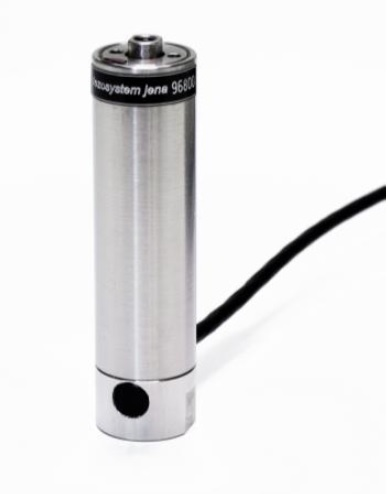
\includegraphics[width=5cm]{Zdjecia/2/piezo_stos}
                \subcaption{\label{subfigure_a}}
        \end{subfigure}
        \begin{subfigure}{0.35\textwidth}
                \centering
	     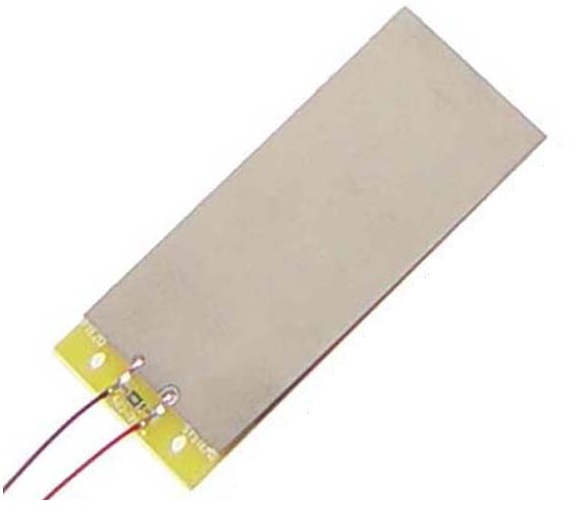
\includegraphics[width=5cm]{Zdjecia/2/piezo_plytka}
                \subcaption{\label{subfigure_b}}
        \end{subfigure}
        \caption{Przetworniki piezoelektryczne: \protect\subref{subfigure_a} w formie sotsu, \protect\subref{subfigure_b} w formie płytki}
        \label{fig:piezoelektryki}
\end{figure}

\vspace{3mm}

Innym sposobem badań jest wykorzystanie techniki laserowej. Za pomocą wiązki lasera możliwe jest wzbudzenie fal sprężystych w materiale. Na szczególną uwagę zasługuje możliwość wzbudzenia fali krótki impulsem, którego widmo będzie miało bardzo duży zakres częstotliwości. Sygnał taki możemy porównać do delty Diraca, dla której widmo ma stałą amplitudę. 

Za pomocą lasera możemy wykonywać także pomiary drgań materiału. Posłużyć może do tego na przykład interferometr laserowy, wykorzystujący efekt Dopplera. Detekcja jest jednak ograniczona do fal powierzchniowych. Atutem takiego pomiaru jest możliwość wykonania go dla wielu punktów na badanym obiekcie. Dzięki temu możemy uzyskać przestrzenny obraz propagacji fali.

Przykładowe stanowisko do badania płyt za pomocą wymuszenia laserem przedstawia rysunek \ref{fig:laser}.

\begin{figure}[h]
\centering
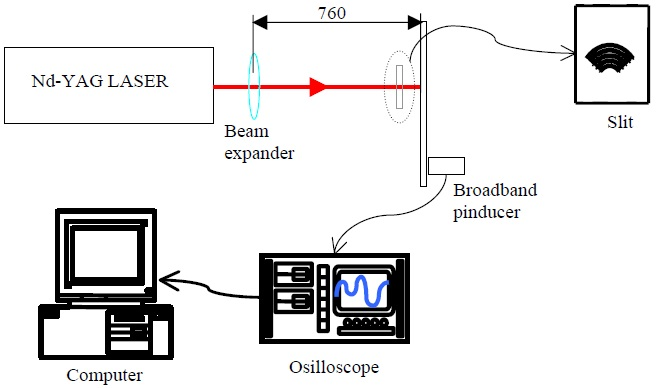
\includegraphics[width=10cm]{Zdjecia/2/laser}
\caption{Przykładowy układ stanowiska do badania fal Lamba w cienkiej płycie \cite{bartek_tian}}
\label{fig:laser}
\end{figure}


%Wzbudzalnosc w sekcji dyspersja

\subsection{Wyznaczanie krzywych wzbudzalności}

Krzywe wzbudzalności określają zależność amplitudy od częstotliwości fali dla poszczególnych jej modów i dla danego wymuszenia. Dla pewnych przypadków można wyznaczyć taką zależność analitycznie, jednak podobnie jak w przypadku krzywych dyspersji, nie jest to metoda uniwersalna. Poniżej znajdują się wyłącznie przykładu numerycznych sposobów wyznaczania tego typu krzywych, ponieważ mają one szersze zastosowanie.

Pierwszy sposób wykorzystuję standardowy model MES ze wzoru \ref{eq:MES1}. Wyznaczamy przemieszczenia węzłów w pewnych chwilach czasowych , a następnie obliczamy wielowymiarowe przekształcenie Fouriera na zgromadzonych danych \ref{eq:fourier_2d}. Wynikiem transformacji jest zależność częstości i liczby falowej, co pozwala wykreślać krzywe dyspersji, a dodatkowo trzecia oś, prostopadła do pozostałych, zawiera informacje o amplitudzie. Przedstawiając na płaszczyźnie zależność amplitudy od liczby falowej, otrzymamy krzywe wzbudzalności.

\vspace{3mm}

Innym sposobem omawianym w literaturze jest zastosowanie metody SAFE (Semi-Analytical Finite Element). Jest ona modyfikacją metody elementów skończonych, polegającą na ustaleniu analitycznego rozwiązania problemu, dla jednego kierunku propagacji. W przypadku problemu trójwymiarowego pozwala to na tworzenie elementów dwuwymiarowych, w kierunkach propagacji, dla których nie znamy rozwiązania. Dzięki temu cały model jest prostszy i szybszy w rozwiązaniu. Sformułowanie takie jest jednak złożone i nie będzie tutaj przytaczane w całości. Jest ono opisane dokładniej w \cite{bartek_fabien}.

Wynikiem wykorzystania metody SAFE jest związek siły wymuszającej i przemieszczenia węzłów modelu. Związek ten przedstawia wzór \ref{eq:wzbudzanie1}. Wzbudzalność określić można na podstawie macierzy E. Określa ona dla modu m, związek pomiędzy siłą przyłożoną w i-tym węźle i przemieszczeniu j-tego węzła \( (\textbf{E}_m)_{ij} \). Rysunek \ref{fig:wzbudzalnosc1} przedstawia wzbudzalność obliczoną dla pierwszych dwóch modów w dwuwarstwowej płycie, bez tłumienia.

\begin{equation} \label{eq:wzbudzanie1}
\textbf{U} = \sum_{m=1}^M \textbf{E}_m \textbf{F}(k_m) e^{ik_m z}
\end{equation}

gdzie
\begin{eqwhere}[2cm]
	\item[$U$] wektor przemieszczenia węzłów
	\item[$E$] macierz wzbudzalności
	\item[$U$] siła wymuszająca w dziedzinie liczby falowej
	\item[$z$] kierunek propagacji, dla którego założono rozwiązanie analityczne
	\item[$m$] numer modu
	\item[$M$] liczba propagujących modów
	\item[$k$] liczba falowa dla m-tego modu.	
\end{eqwhere}

\begin{figure}[h]
\centering
\includegraphics[width=10cm]{Zdjecia/2/wzbudzalnosc1}
\caption{Krzywe wzbudzalności dla dwuwarstwowej cienkiej płyty \cite{bartek_fabien}}
\label{fig:wzbudzalnosc1}
\end{figure}

Kolejna metoda polega na porównaniu prac modów dla fal Lamba z tzw. modem wirtualnym . Prowadzi ona do zależności na wzbudzalność dla cienkich płyt:

\begin{equation} \label{eq:wzbudzanie2}
a_m =  \textbf{X}_m^{(b), H} \frac{\textbf{F}(z)}{i\textbf{P}_{(a:m),(b)}}.
\end{equation}

gdzie

%\begin{equation} \label{eq:wzbudzanie2}
%P_{(a:m),(b)} = \textbf{X}_m^{(b), H} (\textbf{K}_{+1}^{(b),H} e^{-k^{(b)}\Delta x} - \textbf{K}_{-1}^{(b),H} e^{+ik^{(b)}\Delta x} - \textbf{K}_{+1}^{(a)} e^{+ik_m^{(a)}\Delta x} + \textbf{K}_{-1}^{(a)} e^{-ik_m^{(a)}\Delta x})\textbf{X}_{0,m}^{(a)} = 0
%\end{equation}

\begin{equation} \label{eq:wzbudzanie3}
\textbf{P}_{(a:m),(b)} = \textbf{X}_m^{H} (\textbf{K}_{+1}^{H} e^{-ik\Delta x} - \textbf{K}_{-1}^{H} e^{+ik\Delta x} - \textbf{K}_{+1} e^{+ik\Delta x} + \textbf{K}_{-1} e^{-ik\Delta x})\textbf{X}_{0}
\end{equation}

\begin{eqwhere}[2cm]
	\item[$a_m$] amplituda m-tego modu w odpowiedzi na wymuszenie
	\item[$\textbf{F}(z)$] siła wymuszająca działająca wzdłuż grubości płyty
	\item[$\textbf{X}$] wektory własne 
	\item[$\textbf{K}_{\pm 1}$] macierz sztywności dla kolejnej/poprzedniej płaszczyzny propagacji
	\item[$k$] liczba falowa
	\item[$x$] kierunek propagacji
	\item[$m$] numer modu	
	\item[$a_m$] mod numer m, dla pola falowego a
	\item[$b$] mod wirtualny b	
	\item[$H$] sprzężenie hermitowskie.
\end{eqwhere}

Należy zaznaczyć, że do obliczenia amplitud poszczególnych modów, konieczna jest znajomość krzywych dyspersji (zależności \( k(\omega) \) ), oraz wektorów własnych odpowiadających częstościom własnym, dla których wyznaczamy amplitudy.

\subsection{System sing\_around (lub Self-Excited Acoustical System)}

Systemy sing-around to samowzbudne systemy, do pomiaru parametrów rezonansowych fal. Idea systemu polega na dodatnim sprzężeniu zwrotnym pomiędzy przetwornikiem pomiarowym oraz wzbudnikiem. Badanie konstrukcji rozpoczyna arbitralny sygnał wzbudzający. Przetwornik pomiarowy odbiera sygnał i przetwarza go na sygnał elektryczny, który jest odpowiednio filtrowany i wzmacniany, a następnie podawany do wzbudnika. Dane pomiarowe są przesyłane do systemu akwizycji i obróbki, w celu wydobycia informacji o stanie konstrukcji. Schemat przykładowego stanowiska badawczego znajduje się na rysunku \ref{fig:sing_around}.

\begin{figure}[h]
\centering
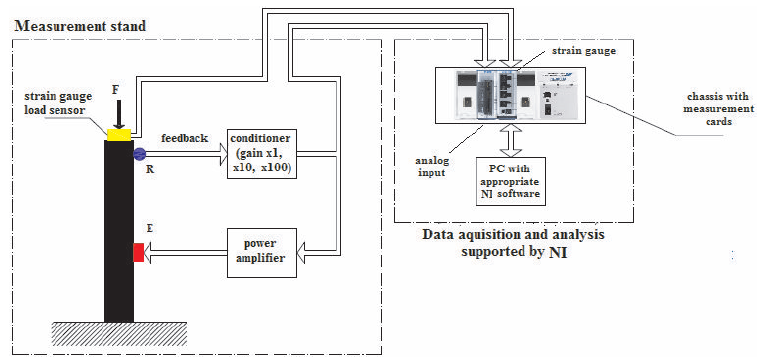
\includegraphics[width=10cm]{Zdjecia/2/sing_around}
\caption{Stanowisko badawcze z systemem sing around \cite{bartek_kwach}}
\label{fig:sing_around}
\end{figure}

Popularnym zastosowaniem tego typu systemów jest pośredni pomiar naprężeń, które mają związek z częstotliwością rezonansową układu bądź prędkością fali, które zmieniają się wraz z odkształcaniem się materiału. Praktycznym przykładem jest pomiar częstotliwości rezonansowej słupa podporowego silosa cementu. Na rysunkach \ref{fig:sing_around_silos} i \ref{fig:sing_around_wyniki} znajduje się widok stanowiska pomiarowego oraz wyniki pomiarów, dla zwiększania i zmniejszania się masy cementu w silosie. W ciągu minuty do silosa dostarczane jest 500kg cementu (125 kg na podporę), a jedno rozładowanie to ok. 2500kg (625 kg na podporę). Przedstawione wyniki dotyczą konfiguracji E1, R1, gdzie E1 to wzbudnik, a R1 to przetwornik pomiarowy.

\begin{figure}[h]
\centering
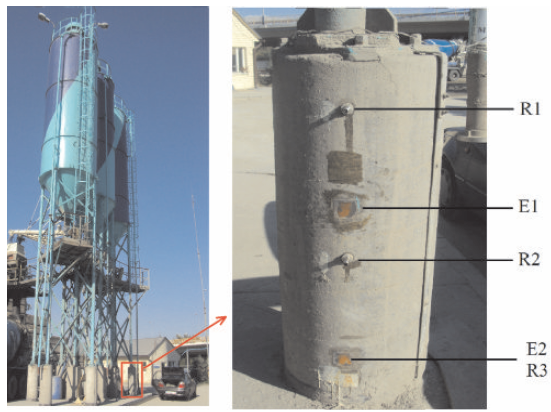
\includegraphics[width=10cm]{Zdjecia/2/sing_around_silos}
\caption{Widok podpory silosa z zamontowanymi przyżadami \cite{bartek_kwach}}
\label{fig:sing_around_silos}
\end{figure}

\begin{figure}[h]
\centering
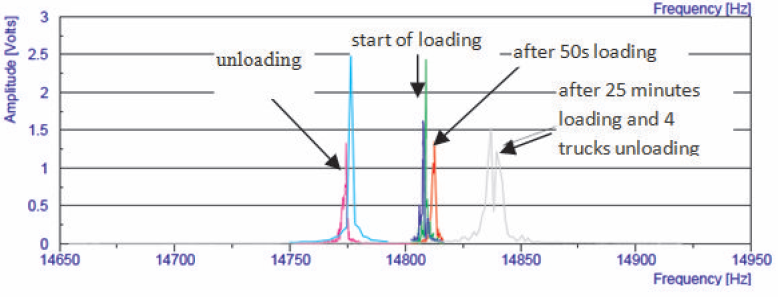
\includegraphics[width=14cm]{Zdjecia/2/sing_around_wyniki}
\caption{Wyniki pomiaru dla ciągłego dostarczania cementu do silosa \cite{bartek_kwach}}
\label{fig:sing_around_wyniki}
\end{figure}

Jak widać częstotliwość rezonansowa zwiększa się wraz ze wzrostem naprężeń ściskających w badanej podporze. Tego typu systemy mają ogromne możliwości zastosowań w różnego typu konstrukcjach, gdzie istotne jest monitorowanie naprężeń.

Znajomość krzywych dyspersji oraz krzywych wzbudzalności dla określonego wymuszenia pozwala zasymulować działanie układu sing-around. Sygnał wyjściowy dla symulacji przebiegu fali, należy podać jako wejście do kolejnej symulacji. Uwzględnienie krzywych dyspersji pozwala określić sposób pomiaru, dla sygnału, który rozbiega się w czasie. Krzywe wzbudzalności pozwalają wyznaczyć piki rezonansowe w widmie badanego sygnału.


%---------------------------------------------------------------------------






















%---------------------------------------------------------------------------





















\chapter{Wykorzystywane zagadnienia metody elementów skończonych}
\chapterauthor{Bartłomiej Piwowarczyk}
\label{cha:MES_chapter}
Metoda elementów skończonych jest zaawansowanym sposobem rozwiązywania równań różniczkowych cząstkowych. Jest ona szczególnym przypadkiem metody Galerkina. Nazwa pochodzi od nazwiska Borisa Grigorievicha Galerkina, który jako pierwszy przeprowadził usystematyzowane studia na temat tego typu metod. Za pomocą tej metody można rozwiązać skomplikowane zadania dziedzin takich jak mechanika ciała stałego, mechanika płynów czy teoria pola elektromagnetycznego. Podstawy tej metody opisane są w \cite{bartek_srodka} oraz \cite{bartek_gavin}. Informacje na temat pochodzenia i estymacji błędów zaczerpnięto z \cite{bartek_pointer} oraz \cite{bartek_erke}.



\section{Rozwiązywanie zadań z  pomocą MES}
\label{sec:rozwiazwyanie_zadan}

W wytrzymałości materiałów poszukujemy zwykle sił działających w poporach konstrukcji i naprężeń wewnątrz jej konkretnych elementów. Innym podejciem jest znalezienie pola przemieszczeń dla każdego punktu konstrukcji.  W jednym i drugim przypadku znalezienie niewiadomych jest osiągalne wyłącznie dla mało skomplikowanych konstrukcji.

Metoda elementów skończonych bierze swoją nazwę od wydzielanych fragmentów konstrukcji, które są właśnie elementami skończonymi. Elementy tworzymy na siatce węzłów, które są punktami wewnątrz lub na brzegach konstrukji. Węzły są także punktami wspólnymi sąsiadujących elementów. Rozwiązanie opiera się na znalezieniu przemieszczenia węzłów i na tej podstawie obliczenia rozwiązania we wszystkich punktach wewnątrz elementów. Kolejne etapy rozwiązywania zadania za pomocą MES przedstawione są poniżej. Rysnuek \ref{fig:MES_przyklad} przedstawia przykład obiektu, który został zdyskretyzowany za pomocą elementów skończonych.

\vspace{5 mm}

\begin{enumerate}
  \item Generacja siatki węzłów.
  \item Budowa elementów skończonych na stworzonej siatce.
  \item Wyznaczanie macierzy mas i sztywności dla każdego elementu (macierze lokalne).
  \item Agregacja macierzy mas  i sztywności dla całej konstrukcji (macierze globalne).
  \item Wprowadzenie wektora obciążeń.
  \item Wprowadzenie warunków brzegowych. Mogą to być siły czynne (modyfikacja wektora obciążeń), naprężenia początkowe czy przemieszczenia wskazanych węzłów.
  \item Rozwiązanie wyznaczonego liniowego równania różniczkowego \( M \ddot x + Kx = F \) - znalezienie przemieszczeń węzłów.
  \item Wyznacznie odkształceń i naprężeń.
  \item Wyznaczenie reakcji w podporach (węzłach, dla których założono przemieszczenie)
\end{enumerate}

\vspace{5 mm}

\begin{figure}[h]
\centering
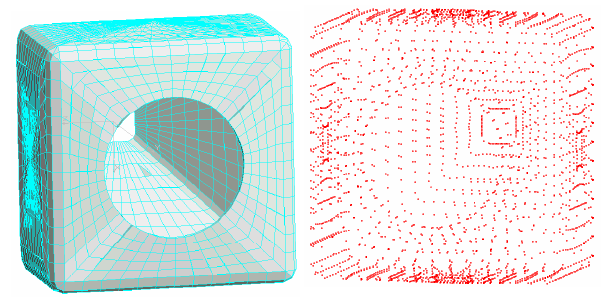
\includegraphics[width=10cm]{Zdjecia/3/MES_przyklad}
\caption{Przykład dsykretyzacji obiektu za pomocą elementów skończonych}
\label{fig:MES_przyklad}
\end{figure}

























\section{Funkcje kształtu}
\label{sec:funkcje_ksztaltu}

Weźmy metalowy pręt o długości L. W punkcie \(x_1\) na pręcie przykładamy temperaturę \( T_1 \), a w punkcie \(x_2\) temperaturę \( T_2 \). Przewidujemy, że po nieskończenie długim czasie rozkład temperatury w pręcie pomiędzy tymi punktami będzie liniowy (Rys. \ref{fig:temperatura_pret}).

\begin{figure}[h]
\centering
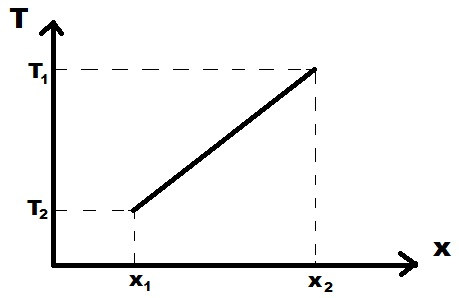
\includegraphics[width=10cm]{Zdjecia/3/rozklad_temperatury}
\caption{Temperatur pomiędzy punktami pręta}
\label{fig:temperatura_pret}
\end{figure}

Temperaturę pomiędzy tymi punktami możemy przedstawić funkcją \ref{eq:funkcja_liniowa}.

\begin{equation} \label{eq:funkcja_liniowa}
T(x)=a_0 + a_1 x, \quad dla \quad x \epsilon [x_1, x_2]
\end{equation}

Można wyznaczyć współczynniki funkcji liniowej mając dwa jej punty.

\begin{equation}
a_1 = \frac{T_2 - T_1}{x_2 - x_1}
\end{equation}

\begin{equation}
a_0 = T_2 - a_1 x_2
\end{equation}

Podstawiając współczyyniki do funkcji, możemy wyznaczyc funkcje kształtu.

\begin{equation}
T(x) = T_1 - \frac{T_2 - T_1}{L} x_1 + \frac{T_2 - T_1}{L} x = \frac{x_2 - x}{L}T_1 + \frac{x - x_1}{L}T_2 = N_1(x)T_1 + N_2(x)T_2
\end{equation}

gdzie
\begin{eqwhere}[2cm]
	\item[$N_1, N_2 $] funkcje kształtu.

\end{eqwhere}

Funkcje kształtu określają w jakim stopniu wartość temperatury z jednego węzła wpływa na wartość temperatury w dowolnym punkcie wewnątrz elementu. Dla większej liczby węzłów w jednowymiarowym elemencie funkcje kształtu są wielomianami wyższych rzędów. Poniżej znajduje się sposób wyznaczania funkcji kształtu na przykładzie 3-węzłowego elementu jednowymiarowego.

\begin{gather} \label{eq:interpolacja}
T(x) = a_0 + a_1 x + a_2 x^2 =
	\begin{bmatrix} 
	 	1 & x& x^2 \\
	\end{bmatrix}
	\begin{bmatrix} 
	 	a_0 \\
		a_1 \\
		a_2 \\
	\end{bmatrix} = \textbf{p} \textbf{a}^e = \textbf{N} \textbf{T}^e
\end{gather}

gdzie
\begin{eqwhere}[2cm]
	\item[$\textbf{p} $] wektor zmiennych kolejnych jednomianów T(x)
	\item[$\textbf{a}^e $] wektor współczynników kolejnych jednomianów T(x)
	\item[$\textbf{N} $] wektor funkcji kształtu
	\item[$\textbf{T}^e $] wektor wartości w węzłach.
\end{eqwhere}

Prawdziwe jest też poniższe równanie.

\begin{gather}
\textbf{T}^e =
	\begin{bmatrix} 
	 	1 & x_1& x_1^2 \\
		1 & x_2& x_2^2 \\
		1 & x_3& x_3^2 \\
	\end{bmatrix}
	\begin{bmatrix} 
	 	a_0 \\
		a_1 \\
		a_2 \\
	\end{bmatrix}
= \textbf{M}^e \textbf{a}^e
\end{gather}

Wyznaczając z tego równania \( \textbf{ a}^e  \) i podstawiając do równania \ref{eq:interpolacja}, otrzymamy następującą zależność.

\begin{equation}
\textbf{p a}^e = \textbf{p} {(\textbf{M}^e)}^{-1} \textbf{T}^e  = \textbf{N T}^e   \quad \Rightarrow \quad \textbf{N} = \textbf{p} {(\textbf{M}^e)}^{-1}
\end{equation}

Funkcje kształtu obliczone w taki sposób mają postać jak poniżej.

\begin{equation}
\begin{aligned}
N_1 = \frac{1}{det\textbf{M}^e} \big(x_2 x_3^2 - x_2^2 x_3 + (x_2^2 - x_3^2)x + (-x_2 + x_3)x^2\big) \\
N_2 = \frac{1}{det\textbf{M}^e} \big(x_1^2 x_3 - x_1 x_3^2 + (x_3^2 - x_1^2)x + (x_1 - x_3)x^2\big) \\
N_3 = \frac{1}{det\textbf{M}^e} \big(x_1 x_2^2 - x_1^2 x_2 + (x_1^2 - x_2^2)x + (-x_1 + x_2)x^2\big)
\end{aligned}
\end{equation}

Prawidłowo wyznaczone funkcje kształtu mają dwi ważną własności. Pierwsza związana jest z węzłami i mówi że każda funkcja przyjmuje wartość 1 w jednym węźle, a we wszystkich pozostałych 0. Druga własność mówi, że suma funkcji kształtu wewnątrz elmentu skończonego wynosi 1. Matematycznie zapisać te własności można następująco:

 \begin{equation} \label{eq:eq_zgodnosc}
	\left\{
                \begin{array}{ll}
		N_n(x_m, y_m) = 1, \quad dla \quad n=m \\
		N_n(x_m, y_m) = 0, \quad dla \quad \neq m 
                \end{array}
	\right.
 \end{equation}

 \begin{equation} \label{eq:WBS}
	\sum_1^n N_n = 1.
 \end{equation}
























\section{Wyznaczanie macierzy sztywności i mas elementów}
\label{sec:wyznaczanie_macierzy}

Weźmy model jednorodnego pręta, obciążonego jak na rysunku \ref{fig:pret} o module Younga \( E \), polu przekroju \( A \) i długości \( L \).

\begin{figure}[h]
\centering
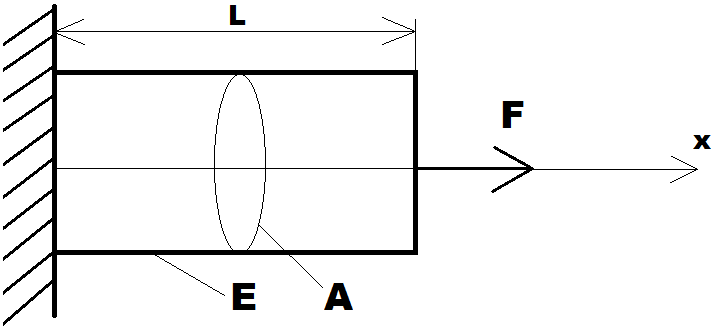
\includegraphics[width=10cm]{Zdjecia/3/pret}
\caption{Model pręta}
\label{fig:pret}
\end{figure}

Energię potencjalną i kinetyczną układu można wyrazić poniższymi wzorami.

\begin{gather} \label{eq:energia}
V = \frac{1}{2} \int_0^L \varepsilon A \sigma dx - Fu_{x=L} = \frac{1}{2} \int_0^L EA {\bigg( \frac{du}{dx}\bigg)}^2 dx - Fu_{x=L} \\
K = \frac{1}{2} \int_0^L \rho A {\bigg(\frac{\partial u}{\partial t}\bigg)}^2 dx
\end{gather}

gdzie
\begin{eqwhere}[2cm]
	\item[$V $] energia potencjalna
	\item[$K $] energia kinetyczna
	\item[$u $] przemieszczenie
	\item[$\varepsilon $] odkształcenie
	\item[$\sigma $] naprężenie
	\item[$F $] siła zewnętrzna skupiona
\end{eqwhere}
	
	Następnie stwórzmy uproszczony model, do którego wyznaczymy zależności MES.

\begin{figure}[h]
\centering
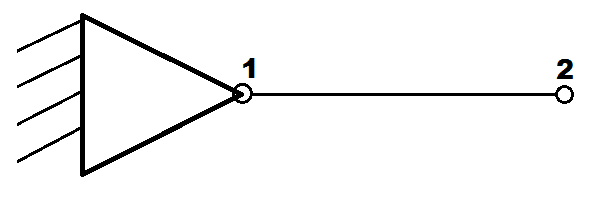
\includegraphics[width=10cm]{Zdjecia/3/pret_upr}
\caption{Uproszczony model pręta}
\label{fig:pret_upr}
\end{figure}

Znając funkcje kształtu i wartości przemieszczeń węzłów można wyznaczyć przemieszczenie w każdym punkcie pręta, a następnie odpowiednie pochodne po przemieszczeniach i po czasie.

\begin{gather}
u = N_1 x_1 + N_2 x_2 = 
	\begin{bmatrix} 
	 	N_1 & N_2 \\
	\end{bmatrix}
	\begin{bmatrix} 
	 	u_1 \\
		u_2 \\
	\end{bmatrix}
\end{gather}

\begin{gather}
\frac{\partial u}{\partial x}= 
	\begin{bmatrix} 
	 	\frac{d N_1}{d x} & \frac{d N_2}{d x} \\
	\end{bmatrix}
	\begin{bmatrix} 
	 	u_1 \\
		u_2 \\
	\end{bmatrix} = \textbf{B u}^e
\end{gather}


\begin{gather}
\frac{\partial u}{\partial t}= 
	\begin{bmatrix} 
	 	N_1 &  N_2 & \\
	\end{bmatrix}
	\begin{bmatrix} 
	 	\frac{du_1}{dt} \\
		\frac{du_2}{dt}\\
	\end{bmatrix} = \textbf{N} \dot{\textbf{u}}^e
\end{gather}


	Mając wyznaczoną energię, możemy obliczyć lagranżjan i wstawić go do dynamicznych równań Lagrangea drugiego rodzaju. Dzięki tej operacji otrzymamy końcowe, dynamiczne równanie ruchu oraz postać macierzy mas i sztywności. Równania Lagrangea drugiego rodzaju mają postać:

\begin{equation}
\frac{d}{dt} \frac{\partial L}{\partial \dot{\textbf{u}}^e} - \frac{\partial L}{\partial \textbf{u}^e} = 0, \quad L = K - V
\end{equation}

gdzie
\begin{eqwhere}[2cm]
	\item[$L$] lagranżjan.
\end{eqwhere}

Pierwszy człon wynosi

\begin{equation}
\frac{d}{dt} \frac{\partial L}{\partial \dot{\textbf{u}}^e} = \int_0^L \rho A {\textbf{N}}^T \textbf{N} {\ddot{\textbf{u}}}^e dx,
\end{equation}

zaś drugi

\begin{equation}
 \frac{\partial L}{\partial \textbf{u}^e} = -\int_0^L EA {\textbf{B}}^T \textbf{B} {\textbf{u}}^e dx + F \textbf{Nu}^e_{x=L}.
\end{equation}

Równanie dynamiki układu zapisane jest poniżej.

\begin{equation}
\int_0^L \rho A {\textbf{N}}^T \textbf{N} dx {\ddot{\textbf{u}}}^e + \int_0^L A {\textbf{B}}^T E \textbf{B} dx u = F \textbf{Nu}^e_{x=L}
\end{equation}

Postaci macierzy mas i sztywności są następujące:

\begin{gather}
\textbf{M}^e = \int_0^L \rho A {\textbf{N}}^T \textbf{N} dx \\
\textbf{K}^e = \int_0^L A {\textbf{B}}^T E \textbf{B} dx.
\end{gather}

W przypadku kiedy występuje więcej niż jedna stała materiałowa, zamiast \( E \) pojawia się macierz materiałowa \( D \). W przypadku bardziej złożonych obiektów o większej liczbie elementów skończonych, całkowanie niezbędne do obliczenia macierzy staje się bardzo czasochłonne. Ponieważ funkcje kształtu są wielomianami, optymalnym rozwiązaniem jest zastosowanie kwadratur Gaussa. Kolejny problem to określenie granic całkowania. W przypadku przedstawionym powyżej nie widać specjalnej trudności, natomiast dla trójwymiarowych obiektów o nieregularnych kształtach wymaga to dodatkowej serii obliczeń.

W takich przypadkach można zastosować mapowanie na współrzędne naturalne. W takich współrzędnych element ma z góry ustalone współrzędne węzłów, co za tym idzie także granice całkowania są znane. Dla obiektu trójwymiarowego przyjmijmy współrzędne rzeczywiste \( x, y, z \) i współrzędne naturalne \( \xi, \eta, \zeta \). Mapowania z jednych współrzędnych na drugie oblicza się według poniższego wzoru. Wizualizacja procedury przedstawiona jest na rysunku \ref{fig:izoparam}.


\begin{gather}
	\begin{bmatrix} 
	 	x \\
		y \\
		z 
	\end{bmatrix} = \sum_{i=1}^n
	\begin{bmatrix} 
	 	x_i \\
		y_i \\
		z_i 
	\end{bmatrix} N_i(\xi, \eta, \zeta)
\end{gather}

\begin{eqwhere}[2cm]
	\item[$x_i, y_i, z_i$] współrzędne rzeczywiste punktów
	\item[$N_i$] funkcje kształtu we współrzędnych naturalnych
	\item[$n$] liczba węzłów elementu.
\end{eqwhere}

\begin{figure}[h]
\centering
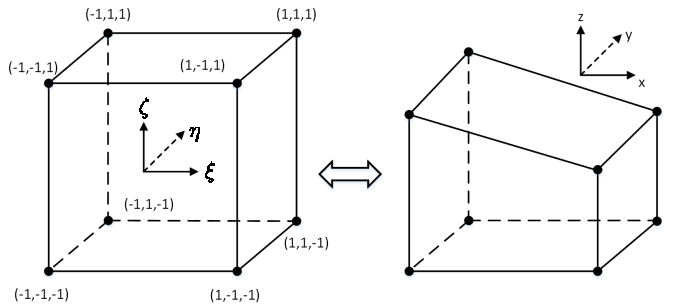
\includegraphics[width=10cm]{Zdjecia/3/izoparam}
\caption{Przekształcenie izoparametryczne}
\label{fig:izoparam}
\end{figure}

Dla elementów w takich współrzędnych funkcje kształtu są znane i stabelaryzowane. Dla elementu sześciennego wypisane są w \ref{eq:f_ksztaltu_hex}.

\begin{equation} \label{eq:f_ksztaltu_hex}
	\begin{aligned}
		N_1 = \frac{1}{8}(1-\xi)(1-\eta)(1-\zeta) \\
		N_2 = \frac{1}{8}(1+\xi)(1-\eta)(1-\zeta) \\
		N_3 = \frac{1}{8}(1+\xi)(1+\eta)(1-\zeta) \\
		N_4 = \frac{1}{8}(1-\xi)(1+\eta)(1-\zeta) \\
		N_5 = \frac{1}{8}(1-\xi)(1-\eta)(1+\zeta) \\
		N_6 = \frac{1}{8}(1+\xi)(1-\eta)(1+\zeta) \\
		N_7 = \frac{1}{8}(1+\xi)(1+\eta)(1+\zeta) \\
		N_8 = \frac{1}{8}(1-\xi)(1+\eta)(1+\zeta)
	\end{aligned}
\end{equation}

Ostatnim elmentem niezbędnym do prawidłowego całkowania we współrzędnych naturalnych jest wyznaczenie jakobianu przekształcenia. Macierz Jacobiego przedstawiona jest w równaniu \ref{eq:m_jacobiego}.

\begin{gather} \label{eq:m_jacobiego}
	\textbf{J} = \begin{bmatrix} 
	 	\frac{\partial x}{\partial \xi} & \frac{\partial y}{\partial \xi} & \frac{\partial z}{\partial \xi} \\
	 	\frac{\partial x}{\partial \eta} & \frac{\partial y}{\partial \eta} & \frac{\partial z}{\partial \eta} \\
	 	\frac{\partial x}{\partial \zeta} & \frac{\partial y}{\partial \zeta} & \frac{\partial z}{\partial \zeta}
	\end{bmatrix}
\end{gather}

Ostatecznie wyznaczanie macierzy mas i sztywności dla elementu sześciennego zostanie zmodyfikowane jak poniżej:

\begin{equation} \label{eq:macierz_sztywnosci}
	\begin{aligned}
	\textbf{K}^e = \int_V {\textbf{B}}^T E \textbf{B} dV \quad \rightarrow \quad \textbf{K}^e =  \int_{-1}^1 \int_{-1}^1 \int_{-1}^1  {\textbf{B}}^T \textbf{D} \textbf{B} det\textbf{J} d\xi d\eta d\zeta.
	\end{aligned}
\end{equation}

\begin{equation} \label{eq:macierz_mas}
	\begin{aligned}
	\textbf{M}^e = \int_V \rho {\textbf{N}}^T \textbf{N} dV \quad \rightarrow \quad \textbf{M}^e = \int_{-1}^1 \int_{-1}^1 \int_{-1}^1 \rho {\textbf{N}}^T \textbf{N} det\textbf{J} d\xi d\eta d\zeta \\
	\end{aligned}
\end{equation}
























\section{Agregacja globalnych macierzy mas i sztywności}
\label{sec:agregacja}

Metoda agregacji macierzy globalnych zostanie przedstawiona na przykładzie macierzy sztywności dwóch elmentów kwadrratowych i obiektu z nich zbudowanego. Wspomniany obiekt przedstawia rysunek \ref{fig:agreg}. Czarne cyfry oznaczają numerację lokalną wewnątrz elmentu, a czerwone numerację globalną.

Algorytm agregacji polega na umieszczaniu odpowiednich elementów macierzy lokalnych do macierzy globalnej. Pokrywające się elementy są sumowane. Ponieważ podmacierz sztywności dla jednego punktu lub zależności pomiędzy punktami jest umieszczana w macierzy globalnej bez wewnętrznych zmian, przyjmijmy zapis uproszczony:

\begin{figure}[h]
\centering
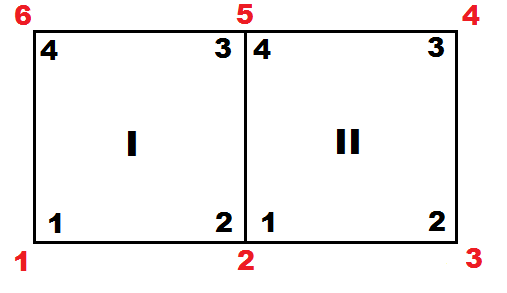
\includegraphics[width=10cm]{Zdjecia/3/agregacja}
\caption{Dwa elementy skończone kwadratowe tworzące obiekt}
\label{fig:agreg}
\end{figure}

\begin{gather}
	\textbf{K}_n^{ij} = \begin{bmatrix} 
	 	K^{ij}_{xx} & K^{ij}_{xy} \\
	 	K^{ij}_{xy} & K^{ij}_{yy} \\
	\end{bmatrix}
\end{gather}

gdzie
\begin{eqwhere}[2cm]
	\item[$i, j$] numery punktów
	\item[$n$] numer elementu
	\item[$x, y$] współrzędne punktów.
\end{eqwhere}

W takim wypadku lokalne macierze sztywności dla obydwu elementów możemy zapisać jako:

\begin{gather}
	\textbf{K}_{I} = \begin{bmatrix} 
	 	\textbf{K}^{11}_I & \textbf{K}^{12}_I & \textbf{K}^{13}_I & \textbf{K}^{14}_I \\
	 	\textbf{K}^{21}_I & \textbf{K}^{22}_I & \textbf{K}^{23}_I & \textbf{K}^{24}_I \\
	 	\textbf{K}^{31}_I & \textbf{K}^{32}_I & \textbf{K}^{33}_I & \textbf{K}^{34}_I \\
	 	\textbf{K}^{41}_I & \textbf{K}^{42}_I & \textbf{K}^{43}_I & \textbf{K}^{44}_I
	\end{bmatrix} \\
	\textbf{K}_{II} = \begin{bmatrix} 
	 	\textbf{K}^{11}_{II} & \textbf{K}^{12}_{II} & \textbf{K}^{13}_{II} & \textbf{K}^{14}_{II} \\
	 	\textbf{K}^{21}_{II} & \textbf{K}^{22}_{II} & \textbf{K}^{23}_{II} & \textbf{K}^{24}_{II} \\
	 	\textbf{K}^{31}_{II} & \textbf{K}^{32}_{II} & \textbf{K}^{33}_{II} & \textbf{K}^{34}_{II} \\
	 	\textbf{K}^{41}_{II} & \textbf{K}^{42}_{II} & \textbf{K}^{43}_{II} & \textbf{K}^{44}_{II}
	\end{bmatrix}.
\end{gather}

Macierze te mają wymiar 8x8, co odpowiada czterem punktom i dwóm współrzędnym dla każdego punktu. Macierz globalna wobec tego będzie miała wymiar 12x12 (6x6 podmacierzy). Poniżej przedstawione jest wyznaczanie kilku elmentów macierzy globalnej.

Dla globalnego punktu 1 mamy:
\begin{equation}
	\textbf{K}^{11} = \textbf{K}_I^{11},
\end{equation}
ponieważ punkt globalny 1 pokrywa się z punktem 1 macierzy I.

Dla globalnego punktu 2 mamy:
\begin{equation}
	\textbf{K}^{22} = \textbf{K}_I^{22} + \textbf{K}_{II}^{11},
\end{equation}
ponieważ punkt globalny 2 pokrywa się z punktem 2 macierzy I oraz punktem 1 macierzy II.

Dla zależności globalnych punktów 2 i 3 mamy:
\begin{equation}
	\textbf{K}^{23} = \textbf{K}_{II}^{12},
\end{equation}
ponieważ punkt globalny 2 pokrywa się z punktem 1, a punkt globalny 3 z punktem 2 macierzy II.

Dla zależności globalnych punktów 2 i 5 mamy:
\begin{equation}
	\textbf{K}^{25} = \textbf{K}_{I}^{23} + \textbf{K}_{II}^{14},
\end{equation}
ponieważ punkt globalny 2 pokrywa się z punktem 2 macierzy I oraz punktem 1 macierzy II, a punkt globalny 5 z punktem 3 macierzy I oraz punktem 4 macierzy II.

Uwzględniając że sztywność względna punktów nie będących ze sobą w sąsiedztwie (np. 1 w pierwszym elemencie oraz 3 w drugim elemencie) wynosi 0, macierz globalna przyjmuje postać:

\begin{gather}
	\textbf{K} = \begin{bmatrix} 
	 	\textbf{K}^{11}_I & \textbf{K}^{12}_I & 0 & 0 & \textbf{K}^{13}_I & \textbf{K}^{14}_I  \\
	 	\textbf{K}^{21}_I & \textbf{K}^{22}_I + \textbf{K}^{11}_{II}  & \textbf{K}^{12}_{II} & \textbf{K}^{13}_II & \textbf{K}_{I}^{23} + \textbf{K}_{II}^{14} & \textbf{K}^{24}_I \\
	 	0 & \textbf{K}^{21}_{II} & \textbf{K}^{22}_{II} & \textbf{K}^{23}_{II} & \textbf{K}^{24}_II & 0 \\
	 	0 & \textbf{K}^{31}_II & \textbf{K}^{32}_{II} & \textbf{K}^{33}_{II} & \textbf{K}^{34}_{II} & 0 \\
		\textbf{K}^{31}_I & \textbf{K}_{I}^{32} + \textbf{K}_{II}^{41} & \textbf{K}^{42}_II & \textbf{K}^{43}_{II} & \textbf{K}^{33}_{I} + \textbf{K}	^{44}_{II} & \textbf{K}^{34}_{I} \\
		\textbf{K}^{41}_I & \textbf{K}^{42}_I & 0 & 0 & \textbf{K}^{43}_I & \textbf{K}^{44}_I.
	\end{bmatrix}
\end{gather}

Oczywistym jest, że w przypadku innej numeracji węzłów globalnych zmieni się układ macierzy globalnej. Nie ma to jednak wpływu na ostateczny wynik rozwiązania MES. W modelach o dużej liczbie elmentów skończonych macierze mas i sztywności są macierzami rzadkimi. Wykorzystuje się to w obliczeniach do oszczędzania pamięci komputera, poprzez zapis w pamięci tylko wartości niezerowych oraz ich położenia w macierzy. 

Macierz mas wyznaczona w przedstawiony sposób jest nazywana macierzą konsystentną. Często stosuje się macierze skupione, które zawierają elementy tylko na diagonali. Pozwala to bardzo przyspieszyć obliczenia. Takie rozwiązanie jest ściśle rzecz biorąc niepoprawne, ponieważ nie ma algorytmu, który pozwala obliczyć macierz skupioną i zachować w pełni właściwości modelu. Macierze skupione oblicza się np. poprzez sumowanie wszystkich elmentów w wierszu i umieszczanie tej sumy na elemencie diagonalnym. Dobrą stroną macierzy skupionych jest fakt, że rozwiązanie pozostaje zbieżne.






















\section{Rozwiązanie wyznaczonego równania macierzowego}
\label{sec:rozwiazanie_r_roz}

Przyjmijmy, że wyznaczone równanie różniczkowe po agregacji macierzy ma postać:

\begin{equation} \label{eq:mes_wyjsciowe}
	\textbf{M} \ddot{\textbf{x}} + \textbf{Kx} = \textbf{F}.
\end{equation}

Rozwiązać to równanie można na wiele sposobów. Przedstawione zostaną tutaj trzy. Pierwszy sposób to metoda całkowania jawnego, druga - metoda całkowania niejawnego, a trzecie to metoda modalna.

W metodzie całkowania jawnego zakładamy rozpoczęcie obliczeń w kroku czasowym t i przybliżamy pochodną drugiego rzędu poprzez formułę centralną:

\begin{equation}
	\ddot{\textbf{x}}^t = \frac{\textbf{x}^{t+1} - 2\textbf{x}^t + \textbf{x}^{t-1}}{\delta t^2}.
\end{equation}

Po podstawieniu do równania \ref{eq:mes_wyjsciowe} wyznaczamy \( \textbf{x}^{t+1} \):

\begin{equation} \label{eq:jawne_calkowanie}
	\textbf{x}^{t+1} = \Delta t^2 \textbf{M}^{-1}(\textbf{F}^t - \textbf{Kx}^t) + 2\textbf{x}^t - \textbf{x}^{t-1}.
\end{equation}

Metoda ta charakteryzuje się tym, że do stabilności rozwiązania często wymaga małego kroku czasowego. Nadaje się ona za to do zrównoleglania obliczeń, co pozwala zastosować do tego celu procesory graficzne. Operacja odwracania macierzy \( \textbf{M} \) we wzorze \ref{eq:jawne_calkowanie} jest kosztowna obliczeniowo. Zastosowanie macierzy skupionej pozwala znacznie przyspieszyć tą procedurę.

Metoda całkowania niejawnego różni się wyjściowym krokiem czasowym. Zakładamy początkową chwilę czasową \( t+1 \), co przy zastosowaniu tej samej formuły różnicowej wprowadza krok wstecz.

\begin{equation} \label{eq:niejawne}
	\ddot{\textbf{x}}^{t+1} = \frac{\textbf{x}^{t+1} - 2\textbf{x}^t + \textbf{x}^{t-1}}{\delta t^2}.
\end{equation}

Podstawiamy równanie \ref{eq:niejawne} do równania

\begin{equation} \label{eq:mes_wyjsciowe}
	\textbf{M} \ddot{\textbf{x}}^{t+1} + \textbf{Kx}^{t+1} = \textbf{F}^{t+1}
\end{equation}

i otrzymujemy 

\begin{equation} 
	\textbf{x}^{t+1} = (\textbf{M} + \Delta t^2 \textbf{K})^{-1} (\Delta t^2 \textbf{F}^{t+1} + 2\textbf{MX}^t - \textbf{MX}^{t-1}.
\end{equation}

W tym wypadku nie unikniemy już odwracania macierzy \( \textbf{M} + \Delta t^2 \textbf{K} \), co powoduje wydłużenie obliczeń. Zaletą tej metody jest fakt, że jest ona bezwarunkowo stabilna.

W metodzie modalnej jako pierwsze należy wyznaczyć wektory własne dla równania jednorodnego \( \textbf{M} \ddot{\textbf{x}} + \textbf{Kx} = 0 \). Wektory własne wyznaczyć można z dokładnością do stałej multiplikatywnej. Możliwe jest wyskalowanie tych wektorów w taki sposób, aby maciesz tych wektorów \( \boldsymbol{\phi} \) miała własność:

\begin{equation} 
	\boldsymbol{\phi}^T \textbf{M} \boldsymbol{\phi} = \textbf{I}.
\end{equation}

Zakładając przekształcenie współrzędnych \( \textbf{x} = \boldsymbol{\phi} \overbar{\textbf{x}}  \) otrzymamy nową postać równania \ref{eq:mes_wyjsciowe}.

\begin{equation} 
	\ddot{\overbar{\textbf{x}}} + \boldsymbol{\Lambda} \overbar{\textbf{x}} = \overbar{\textbf{F}}, \quad \boldsymbol{\Lambda} = \boldsymbol{\phi}^T\textbf{K}\boldsymbol{\phi}, \quad \overbar{\textbf{F}} = \boldsymbol{\phi}^T \textbf{F}.
\end{equation}

Macierz \( \boldsymbol{\Lambda} \) jest macierzą diagonalną, więc rozwiązanie układu sprowadza się teraz do znalezienia rozwiązania dla pojedynczych oscylatorów harmonicznych. Elementy macierzy \( \boldsymbol{\Lambda} \) są kwadratami częstości własnych drgań węzłów.

\begin{gather}
	\begin{bmatrix} 
		\ddot{\overbar{x}_1} \\
		\ddot{\overbar{x}_2} \\
		\ddot{\overbar{x}_3} \\
		\vdots \\
		\ddot{\overbar{x}_n}
	\end{bmatrix} +
	\begin{bmatrix} 
		\omega_1^2	&			&			&				& \\
				& \omega_2^2	& 			& \text{\huge{0}}		& \\
				&			& \omega_3^2 	& 				& \\
				& \text{\huge{0}}	& 			& \ddots			& \\
				&			&			&				& \omega_n^2
	\end{bmatrix}
	\begin{bmatrix} 
		\overbar{x}_1 \\
		\overbar{x}_2 \\
		\overbar{x}_3 \\
		\vdots \\
		\overbar{x}_n
	\end{bmatrix} =
	\begin{bmatrix} 
		\overbar{F}_1 \\
		\overbar{F}_2 \\
		\overbar{F}_3 \\
		\vdots \\
		\overbar{F}_n
	\end{bmatrix}
\end{gather}

 \begin{equation}
	\left\{
                \begin{array}{ll}
  		\ddot{\overbar{x}_1}+\omega_1^2\overbar{x}_1=\overbar{F}_1 \quad \rightarrow\\
  		\ddot{\overbar{x}_2}+\omega_2^2\overbar{x}_2=\overbar{F}_2 \quad \rightarrow\\
  		\ddot{\overbar{x}_3}+\omega_3^2\overbar{x}_3=\overbar{F}_3 \quad \rightarrow\\
		\quad \quad \vdots \quad \quad \\
  		\ddot{\overbar{x}_n}+\omega_n^2\overbar{x}_n=\overbar{F}_n \quad \rightarrow
                \end{array}
	\begin{bmatrix} 
		\overbar{x}_1 \\
		\overbar{x}_2 \\
		\overbar{x}_3 \\
		\vdots \\
		\overbar{x}_n
	\end{bmatrix}
	\right.
 \end{equation}

Po rozwiązaniu równań należy wyznaczyć ostateczne rozwiązanie \( \textbf{x} = \boldsymbol{\phi} \overbar{\textbf{x}}  \).




















\section{Zbieżność metody i błędy rozwiązania}
\label{sec:zbieznosc_i_blad}

O zbieżności rozwiązania możemy wnioskować na podstawie funkcji kształtu. Pierwszym warunkiem jest tzw. warunek zgodności. Mówi on o tym, że funkcje kształtu muszą być ciągłe w przestrzeni elementów. Dla prostego przypadku dwóch elementów liniowych jednowymiarowych ciągłość funkcji ilustruje rysunek \ref{fig:zgodnosc}. 

\begin{figure}[h]
\centering
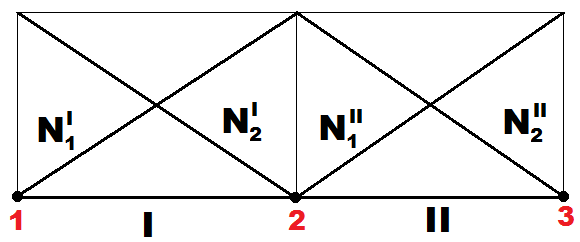
\includegraphics[width=10cm]{Zdjecia/3/zgodnosc}
\caption{Ciągłość funkcji w przestrzenii elementów}
\label{fig:zgodnosc}
\end{figure}

Warunek ten jest zapewniony poprzez własność funkcji kształtu przedstawioną we wzorze \ref{eq:eq_zgodnosc}.

Kolejny warunek nazywa się warunkiem bryły sztywnej (WBS). Zapewnia on brak straty bądź narastania energii podczas wyznaczania wyniku wewnątrz elementu. Warunek ten jest zapewniony poprzez własność funkcji kształtu przedstawioną w \ref{eq:WBS}.

Ostatnim warunkiem jest tzw. warunek stałego odkształcenia (WSO). Mówi on o tym, że jeśli w elemencie przyłożymy liniowe pole przemieszczeń, to odkształcenie będzie stałe w każdym punkcie elementu.

Jeśli spełnione są warunki zgodności, WBS oraz WBO to rozwiązanie dla elementu będzie zbieżne. Warunki te muszą być spełnione dla każdego elementu obliczanego modelu.

\vspace{3mm}

Zbieżność nie daje nam gwarancji, że rozwiązanie otrzymane przy pomocy symulacji MES jest poprawne. Przez poprawne rozumiane jest, że błąd rozwiązania jest dostatecznie mały. Aby mieć pewność, że rozwiązanie jest wystarczająco dokładne należy oszacować błąd maksymalny. W przypadku MES błąd powodują:

\begin{enumerate}
	\item dyskretyzacja konstrukcji 
	\item zaokrąglenia arytmetyczne.
\end{enumerate}

\vspace{3mm}

Pierwsza przyczyna występowania błędów związana jest z podziałem konstrukcji na elementy skończone. Błąd zawarty jest już w równaniu \( \textbf{M} \ddot{\textbf{x}} + \textbf{Kx} = \textbf{F} \). Pojawia się dlatego, że całe rozwiązanie wyznaczamy za pomocą wielomianowych funkcji kształtu. Błąd zbieżnego rozwiązania możemy zmniejszać poprzez wykorzystanie funkcji kształtu wyższego rzędu, bądź zagęszczenie siatki i budowę większej liczby elementów skończonych.

Estymacja błędów odbywa się na różne sposoby. Jednym z nich jest wykorzystanie równania \ref{eq:blad1}. 

\begin{equation} \label{eq:blad1}
	F - \tilde{F}_i \approx ch_i^r
\end{equation}

gdzie
\begin{eqwhere}[2cm]
	\item[$ F $] rozwiązanie dokładne
	\item[$ \tilde{F}_i $] i-te rozwiązanie przybliżone
	\item[$ c $] współczynnik proporcjonalności
	\item[$ h_i $] współczynnik zależny od zagęszczenia siatki
	\item[$ r $] współczynnik zależny od stopnia wielomianów interpolujących.
\end{eqwhere}

Jedna symulacja nie daje możliwości wyznaczyć błędu. Aby tego dokonać należy przeprowadzić dwie symulacje, co pozwala obliczyć błąd drugiej (dokładniejszej). Przyjmijmy, że druga symulacja zawiera elementy o dwukrotnie mniejszych wymiarach, czyli \( h_1 = 2h_2 \). Współczynnik \( r \) przyjmuje wartości mniejsze od 1, ale dla uproszczenia przyjmijmy dokładnie 1.

Podstawiając odpowiednie indeksy do wzoru \ref{eq:blad1}, możemy wyznaczyć błąd drugiej symulacji, znając wyniki zarówno pierwszej jak i drugiej.

\begin{equation} 
	F- \tilde{F}_2 \approx \frac{\tilde{F}_2 - \tilde{F}_1}{(\frac{h_1}{h_2})^r - 1}.
\end{equation}

Innym podejściem jest wyznaczanie błędów poprzez energię naprężenia elementów. Po wyznaczeniu przemieszczeń węzłów i obliczeniu naprężeń, naprężenia nie są ciągłe w przestrzeni elementów. Jeśli jeden węzeł należy do kilku elementów, to w każdym z nich może zostać wyznaczona inna wartość naprężenia dla takiego węzła. W ciągłym przypadku naprężenie byłoby funkcją ciągłą, dlatego błąd wynikający z naprężeń wyznacza się w następujący sposób:

\vspace{3mm}

\begin{enumerate}
	\item Obliczamy średnią naprężeń w węźle, biorąc wartości dla węzła z każdego elementu, do którego należy.
	\item Wyznaczamy błąd naprężenia w węzłach elementu, poprzez odejmowanie od naprężenia w węźle wartości średniego naprężenia w tym węźle.
	\item Sumujemy błędy naprężeń wszystkich elementów skończonych.
	\item Wyznaczamy energię błędu naprężenia.
	\item Wyznaczamy energię odkształcenia dla całej konstrukcji.
	\item Obliczamy błąd procentowy według wzoru \ref{eq:blad2}.
\end{enumerate}

\vspace{3mm}

\begin{equation} \label{eq:blad2}
	E = 100(\frac{e}{U + e})^{0.5}
\end{equation}

gdzie
\begin{eqwhere}[2cm]
	\item[$ e $] całkowita energi błędu dla konstrukcji
	\item[$ U $] energi odkształcenia dla konstrukcji
	\item[$ E $] błąd procentowy energii.
\end{eqwhere}












































%\chapter{Aplikacja do obliczeń numerycznych}
\label{cha:aplikacja_do_obliczen_numerycznych}

\LaTeX~jest systemem składu umożliwiającym tworzenie dowolnego typu dokumentów (w~szczególności naukowych i technicznych) o wysokiej jakości typograficznej (\cite{Dil00}, \cite{Lam92}). Wysoka jakość składu jest niezależna od rozmiaru dokumentu -- zaczynając od krótkich listów do bardzo grubych książek. \LaTeX~automatyzuje wiele prac związanych ze składaniem dokumentów np.: referencje, cytowania, generowanie spisów (treśli, rysunków, symboli itp.) itd.

\LaTeX~jest zestawem instrukcji umożliwiających autorom skład i wydruk ich prac na najwyższym poziomie typograficznym. Do formatowania dokumentu \LaTeX~stosuje \TeX a (wymiawamy 'tech' -- greckie litery $\tau$, $\epsilon$, $\chi$). Korzystając z~systemu składu \LaTeX~mamy za zadanie przygotować jedynie tekst źródłowy, cały ciężar składania, formatowania dokumentu przejmuje na siebie system.

%---------------------------------------------------------------------------

\section{Cele pracy}
\label{sec:celePracy}


Celem poniższej pracy jest zapoznanie studentów z systemem \LaTeX~w zakresie umożliwiającym im samodzielne, profesjonalne złożenie pracy dyplomowej w systemie \LaTeX.

\subsection{Jakiś tytuł}

\subsubsection{Jakiś tytuł w subsubsection}


\subsection{Jakiś tytuł 2}

%---------------------------------------------------------------------------

\section{Zawartość pracy}
\label{sec:zawartoscPracy}

W rodziale~\ref{cha:pierwszyDokument} przedstawiono podstawowe informacje dotyczące struktury dokumentów w \LaTeX u. Alvis~\cite{Alvis2011} jest językiem 



















%\chapter{Pomiary}
\label{cha:pomiary}

\LaTeX~jest systemem składu umożliwiającym tworzenie dowolnego typu dokumentów (w~szczególności naukowych i technicznych) o wysokiej jakości typograficznej (\cite{Dil00}, \cite{Lam92}). Wysoka jakość składu jest niezależna od rozmiaru dokumentu -- zaczynając od krótkich listów do bardzo grubych książek. \LaTeX~automatyzuje wiele prac związanych ze składaniem dokumentów np.: referencje, cytowania, generowanie spisów (treśli, rysunków, symboli itp.) itd.

\LaTeX~jest zestawem instrukcji umożliwiających autorom skład i wydruk ich prac na najwyższym poziomie typograficznym. Do formatowania dokumentu \LaTeX~stosuje \TeX a (wymiawamy 'tech' -- greckie litery $\tau$, $\epsilon$, $\chi$). Korzystając z~systemu składu \LaTeX~mamy za zadanie przygotować jedynie tekst źródłowy, cały ciężar składania, formatowania dokumentu przejmuje na siebie system.

%---------------------------------------------------------------------------

\section{Cele pracy}
\label{sec:celePracy}


Celem poniższej pracy jest zapoznanie studentów z systemem \LaTeX~w zakresie umożliwiającym im samodzielne, profesjonalne złożenie pracy dyplomowej w systemie \LaTeX.

\subsection{Jakiś tytuł}

\subsubsection{Jakiś tytuł w subsubsection}


\subsection{Jakiś tytuł 2}

%---------------------------------------------------------------------------

\section{Zawartość pracy}
\label{sec:zawartoscPracy}

W rodziale~\ref{cha:pierwszyDokument} przedstawiono podstawowe informacje dotyczące struktury dokumentów w \LaTeX u. Alvis~\cite{Alvis2011} jest językiem 



















%\chapter{Porównanie metod i wnioski}
\label{cha:porownanie_metod_i_wnioski}

\LaTeX~jest systemem składu umożliwiającym tworzenie dowolnego typu dokumentów (w~szczególności naukowych i technicznych) o wysokiej jakości typograficznej (\cite{Dil00}, \cite{Lam92}). Wysoka jakość składu jest niezależna od rozmiaru dokumentu -- zaczynając od krótkich listów do bardzo grubych książek. \LaTeX~automatyzuje wiele prac związanych ze składaniem dokumentów np.: referencje, cytowania, generowanie spisów (treśli, rysunków, symboli itp.) itd.

\LaTeX~jest zestawem instrukcji umożliwiających autorom skład i wydruk ich prac na najwyższym poziomie typograficznym. Do formatowania dokumentu \LaTeX~stosuje \TeX a (wymiawamy 'tech' -- greckie litery $\tau$, $\epsilon$, $\chi$). Korzystając z~systemu składu \LaTeX~mamy za zadanie przygotować jedynie tekst źródłowy, cały ciężar składania, formatowania dokumentu przejmuje na siebie system.

%---------------------------------------------------------------------------

\section{Cele pracy}
\label{sec:celePracy}


Celem poniższej pracy jest zapoznanie studentów z systemem \LaTeX~w zakresie umożliwiającym im samodzielne, profesjonalne złożenie pracy dyplomowej w systemie \LaTeX.

\subsection{Jakiś tytuł}

\subsubsection{Jakiś tytuł w subsubsection}


\subsection{Jakiś tytuł 2}

%---------------------------------------------------------------------------

\section{Zawartość pracy}
\label{sec:zawartoscPracy}

W rodziale~\ref{cha:pierwszyDokument} przedstawiono podstawowe informacje dotyczące struktury dokumentów w \LaTeX u. Alvis~\cite{Alvis2011} jest językiem 



















%\chapter{Podsumowanie}
\label{cha:podsumowanie}

\LaTeX~jest systemem składu umożliwiającym tworzenie dowolnego typu dokumentów (w~szczególności naukowych i technicznych) o wysokiej jakości typograficznej (\cite{Dil00}, \cite{Lam92}). Wysoka jakość składu jest niezależna od rozmiaru dokumentu -- zaczynając od krótkich listów do bardzo grubych książek. \LaTeX~automatyzuje wiele prac związanych ze składaniem dokumentów np.: referencje, cytowania, generowanie spisów (treśli, rysunków, symboli itp.) itd.

\LaTeX~jest zestawem instrukcji umożliwiających autorom skład i wydruk ich prac na najwyższym poziomie typograficznym. Do formatowania dokumentu \LaTeX~stosuje \TeX a (wymiawamy 'tech' -- greckie litery $\tau$, $\epsilon$, $\chi$). Korzystając z~systemu składu \LaTeX~mamy za zadanie przygotować jedynie tekst źródłowy, cały ciężar składania, formatowania dokumentu przejmuje na siebie system.

%---------------------------------------------------------------------------

\section{Cele pracy}
\label{sec:celePracy}


Celem poniższej pracy jest zapoznanie studentów z systemem \LaTeX~w zakresie umożliwiającym im samodzielne, profesjonalne złożenie pracy dyplomowej w systemie \LaTeX.

\subsection{Jakiś tytuł}

\subsubsection{Jakiś tytuł w subsubsection}


\subsection{Jakiś tytuł 2}

%---------------------------------------------------------------------------

\section{Zawartość pracy}
\label{sec:zawartoscPracy}

W rodziale~\ref{cha:pierwszyDokument} przedstawiono podstawowe informacje dotyczące struktury dokumentów w \LaTeX u. Alvis~\cite{Alvis2011} jest językiem 




















%\include{tests}

%Kod poniżej dodaje Bibliografię do spisu treści
\cleardoublepage
\phantomsection
\addcontentsline{toc}{chapter}{Bibliografia}
\printbibliography

% Załączniki
\begin{appendices}
  \makeatletter% Kod poniżej powoduje ustęp w spisie treści
  \addtocontents{toc}{\let\protect\l@chapter\protect\l@section}
  \chapter{Lorem Ipsum}

Lorem ipsum dolor sit amet, consectetur adipiscing elit. Fusce aliquet consequat sollicitudin. Nam nec eros ut dolor vulputate maximus. Vivamus quis neque sed orci cursus ornare. Proin vel elit eros. Duis efficitur mi tempus mi volutpat ullamcorper. Vestibulum consectetur dictum dui, ac suscipit eros aliquet ac. Quisque at dignissim mauris. Nulla non finibus nunc. In hac habitasse platea dictumst. Donec semper in nunc eget ultricies. Fusce varius scelerisque cursus. Vestibulum a sem lobortis, pretium nibh quis, pharetra justo.

Mauris turpis nunc, dignissim ac fringilla quis, dignissim sed dui. Cras porttitor congue nulla, vitae hendrerit ligula hendrerit vel. Donec lorem lectus, tempor a feugiat et, ultrices at augue. Suspendisse ultricies massa vitae pellentesque accumsan. Phasellus sollicitudin hendrerit lorem, lobortis aliquet nibh tristique a. Etiam nec tempus enim. Aenean diam nibh, pretium tincidunt malesuada vitae, laoreet non orci. Fusce dictum feugiat eros in malesuada. Sed vel ligula nunc. Donec nec hendrerit mauris. Sed accumsan quis quam vitae interdum. Praesent nec arcu est. Donec cursus nisi vitae ligula pharetra, quis sagittis felis dignissim.

Nunc a dapibus elit, nec iaculis erat. Suspendisse eleifend neque ac odio volutpat vulputate. Etiam varius odio quis leo aliquam, ac laoreet turpis vulputate. Donec rutrum pulvinar odio, vitae maximus ipsum bibendum a. Curabitur euismod erat a cursus vehicula. Aenean quis quam vulputate, consequat erat vitae, molestie felis. Morbi gravida nulla vitae leo hendrerit iaculis. Donec lobortis, quam ac ultrices aliquam, purus lectus tempus enim, et dictum nunc tortor vitae ligula. Aliquam volutpat bibendum nulla, non elementum nunc congue ut. Aenean mattis arcu in velit faucibus, vel eleifend nibh imperdiet. Etiam eget gravida nulla, quis varius sapien.

Donec bibendum commodo mi, vel interdum neque mattis nec. Suspendisse potenti. In lectus elit, accumsan non purus quis, viverra eleifend ipsum. Sed vel ex sed dolor consectetur scelerisque. Praesent id leo ultrices eros ornare accumsan. Mauris pharetra justo at tortor scelerisque mattis. Quisque eu risus vitae mi tristique pulvinar eget et nisi. Praesent a nibh vitae nunc aliquet laoreet eu eu massa. Sed aliquet mollis cursus. In erat nisl, suscipit eget justo id, euismod pellentesque nulla.
  % \input{zalocznikB}
  % itd.
  \makeatother%
\end{appendices}

\end{document}
